\chapter{Simulation and Results}
\label{chap:5_Simulation_And_Results}
    
        %V1.0:
        % In this chapter, we present scenarios for validation and evaluation and experimental results. The scenarios cover different encounters between vessels for collision avoidance evaluation and for identification of our system's response and limitations we expose it to different wind speeds. Beyond that, we present the execution with and without \ac{\ac{ATC}} for scientific control validation of the path planning algorithm. As done by several authors, \eg{} Larson \etal{} ~\cite{Larson2006Autonomous}, Naeem \etal{} ~\cite{Naeem2012COLREGS}, Campbell \etal{} ~\cite{Campbell2013Automatic}, Naus ~\cite{Naus2013Idea}, \etc{}, we evaluated 4 main encounter scenarios between two vessels: head-on, crossing from right, crossing from left and overtaking. Based on \cite{} we made a quantitative evaluation of our planning system measuring computational cost and minimum distance between vessels.
        
        %V2.0:
        % In this chapter, we present scenarios for validation (qualitative analysis) and evaluation (quantitative analysis) and experimental results. The scenarios cover different encounters between vessels for collision avoidance success evaluation and exposition to different environmental behaviors for identification of response capability and limitations of our system. Beyond that, we present the execution with and without \ac{\ac{ATC}} for scientific control validation of our path planning algorithm.
        
        %V3.0:
        % In this chapter, we present the scenarios for validation (qualitative analysis) and evaluation (quantitative analysis) and experimental results. The scenarios cover different encounters between vessels for collision avoidance success evaluation and exposition to different environmental behaviors for identification of response capability and limitations of our system. Beyond that, we present the execution of our path planning algorithm with and without \ac{\ac{ATC}}.
        
        %V4.0:
        % In this chapter, we present the scenarios for validation (qualitative analysis) and evaluation (quantitative analysis) of our approach, as well as the experimental results. The simulations cover different encounters scenarios between vessels for evaluation of collision avoidance success and exposition to different environmental behaviors for identification of limitations of our system.
        
        %V5.0:
        % In this chapter, we present the scenarios for qualitative and quantitative evaluation of our approach, as well as the experimental results. The simulations cover different encounters scenarios between vessels for evaluation of collision avoidance success and exposition to different environmental behaviors for identification of limitations of our system.
        
        % V6.0:
        % In this chapter, we present the simulation scenarios for qualitative and quantitative evaluation of our systems, as well as the experimental results. The simulations cover different encounters scenarios between vessels, this way we evaluate collision avoidance success and the behavior of our system when exposed to different environment conditions.
        
        % V7.0:
        % Grammarlly: 100/100
        In this chapter, we present simulation scenarios for qualitative and quantitative evaluation of our system, as well as the experimental results. The simulations cover different encounters scenarios between two vessels, one using our path planning method and other without any COLREGS-compliant method. For qualitative evaluation, we analyzed avoidance success and the behavior of our system when exposed to different environmental conditions. For quantitative evaluation, we analyzed the time for computation of our path planning method and the minimum distance kept between our COLREGS-compliant vessel and the encountering vessel during the simulation.

    \section{Simulations Characterization}

    % Grammarlly: 100/100
    We run our simulations on \usvsim ~\cite{Paravisi2018Toward} simulator using the platform described in Table \ref{tab:simulation_platform_description}. 
    We developed 12 scenarios for evaluation the system focusing on being comparable with simulations presented in reference studies, \ie{} Agrawal \etal{} ~\cite{Agrawal2015COLREGS} and Huang \etal{} ~\cite{Huang2019Generalized}. We chose both studies for their quality (\ie{} h-index) and similarity with our work. Agrawal \etal{} present our problem-solving inspiration but unfortunately, they do not present too much information about their system evaluation, so we based our tests and system evaluation on Huang \etal{} as they explicitly present their simulation scenarios characterization, results, and simulate a \ac{USV} similar to ours in the aspect of dimensions.
    
    \taburowcolors[1] 1{tableLineOne .. tableLineTwo}
    \tabulinesep = ^3mm_2mm
    \everyrow{\tabucline[.4mm  white]{}}

    \begin{table}[H]
        \caption{Simulation Platform Description}
        \centering
            \begin{tabu} to \textwidth { >{\bfseries}X[c, 0] X[c, 3]}
            \tableHeaderStyle
            Component & Specification \\
            Computer & Desktop Dell XPS 8700 \\
            Processor & Intel® Core™ i7-4770 CPU @ 3.40GHz × 8 \\
            Memory & \begin{tabular}[c]{@{}l@{}}Teikon PC3-12800u DDR3 1600 MHz 2GB x 2\\ Teikon PC3-12800u DDR3 1600 MHz 4GB x 2\end{tabular} \\
            Operating System & Ubuntu 16.04.6 LTS \\
            ROS Version & ROS Kinetic
            \end{tabu}  
        \label{tab:simulation_platform_description}
    \end{table}
    
    % Grammarlly: 100/100
    In our simulations, we use a differential boat - shown in Figure \ref{fig:diffboat} - with two thrusters, which enables it to rotate over its axis. This boat is modeled according to specifications of the Lutra Prop boat, acquired from Platypus ~\cite{PlatypusLLC}. Beyond the specifications shown in Table \ref{tab:diffboat_specs}, the Lutra boat we use in our simulation has a laser rangefinder for environment scanning in its bow. We set the rangefinder to be capable of detect objects in 25 meters in a range of 360°.
%AMA acho q apresentacao do barco deva vir antes da apresentacao dos 4 cenarios. vc deve mencionar outras caracteristicas, como peso, sensores, a caracteristicas do laser.  
%DJ:    1- Boat: Done; 
%       2 - Outras caracteristicas: Done
    
    % \taburowcolors[1] 1{tableLineOne .. tableLineTwo}
    % \tabulinesep = ^3mm_2mm
    % \everyrow{\tabucline[.4mm  white]{}}
    % \begin{table}
    %     \caption{Lutra Prop parameters}
    %     \centering
    %         \begin{tabu} to 0.45\textwidth { >{\bfseries}X[c, 2] X[c, 2]}
    %         \tableHeaderStyle
    %         Parameter       & Value       \\
    %         Length          & 106 cm      \\
    %         Width           & 48 cm       \\
    %         Height          & 15 cm       \\
    %         % Hull Volume     & ~0.02 $m^3$ \\
    %         Weight          & 9.7 Kg      \\
    %         % Extra Payload   & 3 Kg        \\
    %         % Thruster Force  & 22.54 N     \\
    %         % Linear drag     & 11.33       \\
    %         Maximum speed   & 1.41 m/s    \\
    %         \end{tabu}  
    %     \label{tab:simulation_platform_description}
    % \end{table}
    
    \begin{minipage}{\textwidth}
        \begin{minipage}[b]{0.35\textwidth}
        \centering
        \begin{figure}[H]
            \centering
            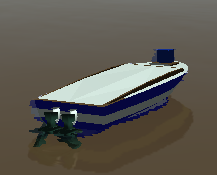
\includegraphics[scale=0.75]{figs/Chap5/diffboat.png}
            % \caption{Simulated version of Lutra Prop boat}
            % \label{fig:diffboat}
        \end{figure}
        \captionof{figure}{Simulated version of Lutra Prop boat}
        \label{fig:diffboat}
        \end{minipage}
    %   \hfill
        \begin{minipage}[b]{0.5\textwidth}
        \centering
            \begin{tabular}{cc}
                \toprule
                    \textbf{Parameter}       & \textbf{Value}       \\
                \midrule
                    Length          & 106 cm      \\
                    Width           & 48 cm       \\
                    Height          & 15 cm       \\
                    Weight          & 9.7 Kg      \\
                    Maximum speed   & 1.41 m/s    \\ 
                \bottomrule
            \end{tabular}
        \captionof{table}{Lutra Prop parameters}
        \label{tab:diffboat_specs}
        \end{minipage}
    \end{minipage}
    
    \vskip 1cm
    
     We assembled the scenarios in a simulated version of the Dilúvio stream (see Figures , \ref{fig:simulation_diluvio_googleLocation2_1_roundedArea} \ref{fig:simulation_diluvio_googleLocation2_2_roundedArea} and \ref{fig:simulation_diluvio_googleLocation_roundedArea}). As done by several authors, \eg{} Larson \etal{} ~\cite{Larson2006Autonomous}, Naeem \etal{} ~\cite{Naeem2012COLREGS}, Campbell \etal{} ~\cite{Campbell2013Automatic}, Naus ~\cite{Naus2013Idea}, \etc{}, we evaluated 4 main encounter scenarios between two vessels, head-on, crossing from right, crossing from left, and overtaking. Figures \ref{fig:simulation_uwsim_headon_starting_pos}, \ref{fig:simulation_uwsim_crossingright_starting_pos}, \ref{fig:simulation_uwsim_crossingleft_starting_pos} and \ref{fig:simulation_uwsim_overtake_starting_pos} show the starting configuration of the evaluated scenarios, the respective configuration of each scenario is presented in Tables \ref{tab:simulation_scenarios_configuration_own_vessel} and \ref{tab:simulation_scenarios_configuration_encountering_vessel}.
    
    \begin{figure}[H]
    \centering
        \begin{subfigure}[b]{0.5\textwidth}
            \centering
            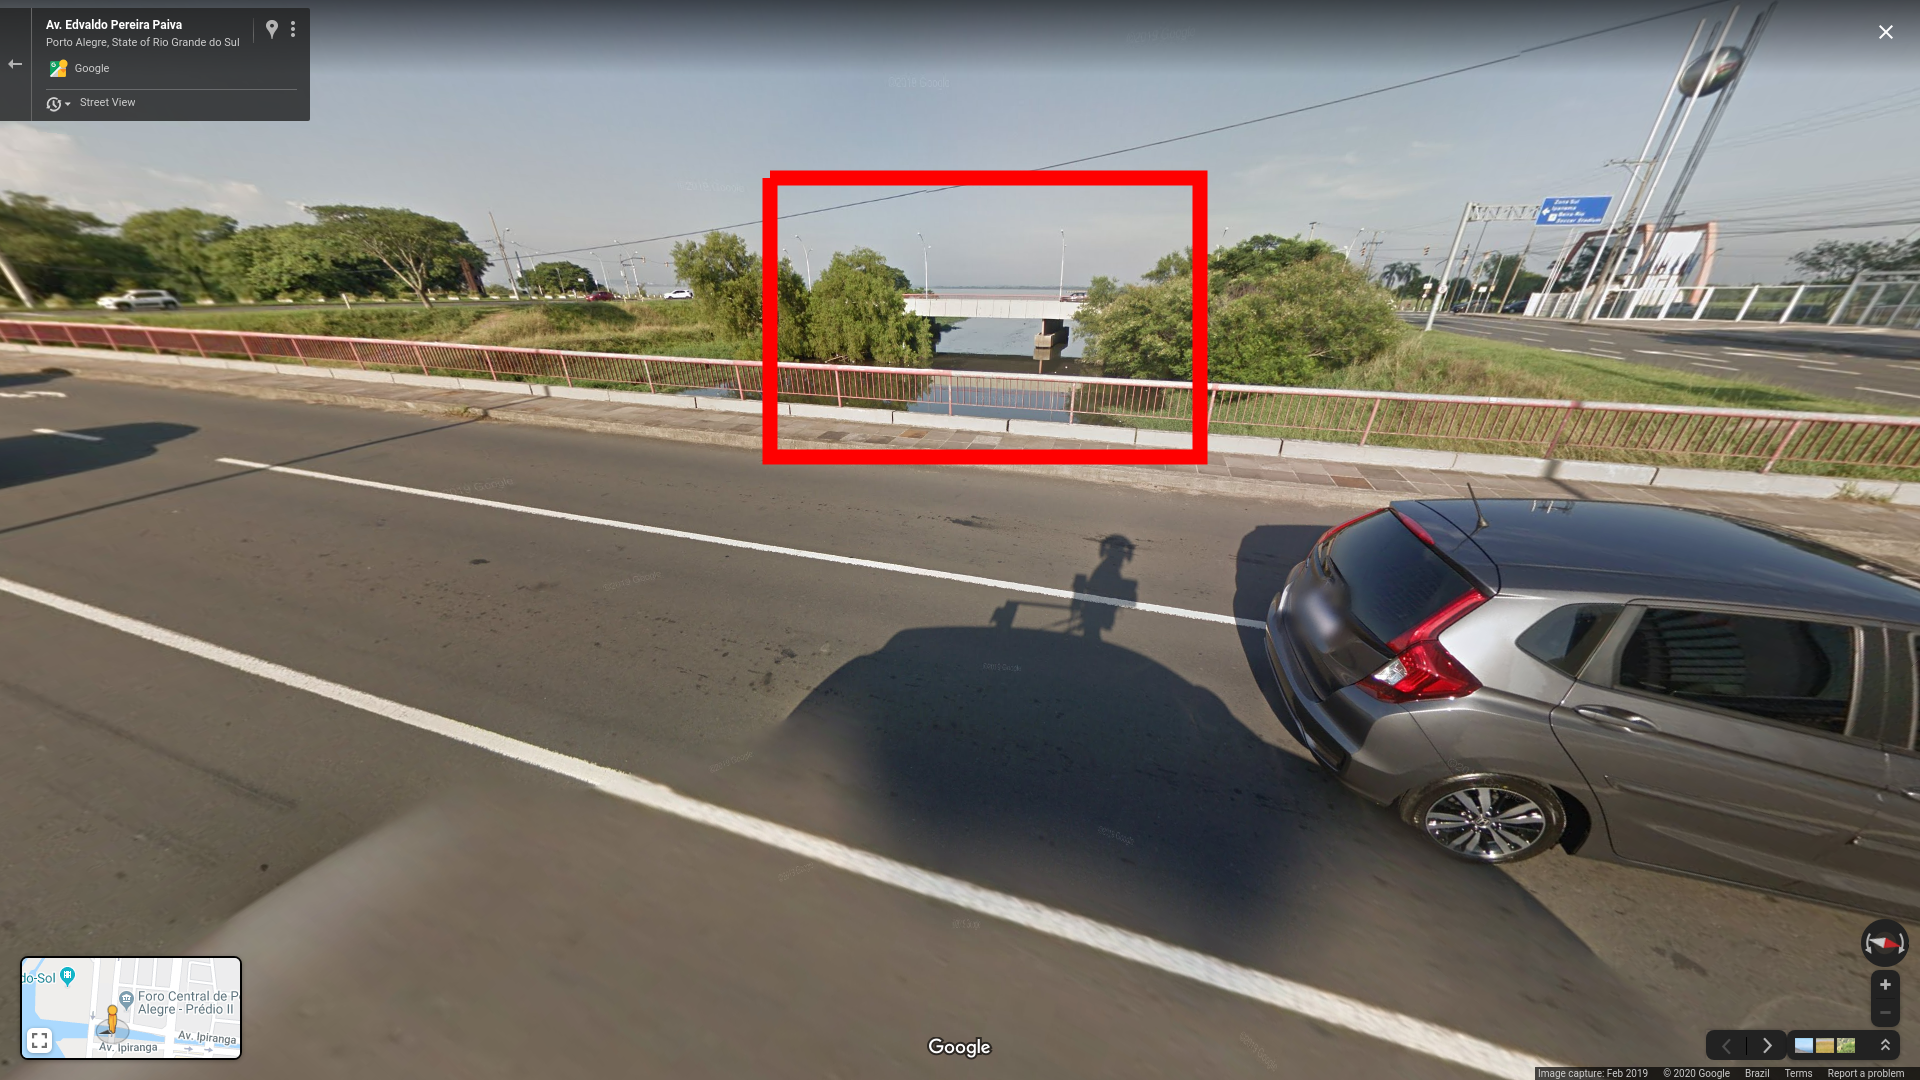
\includegraphics[scale=0.12]{figs/Chap5/simulation_diluvio_googleLocation2_1_roundedArea.png}
            \caption{Real World Location}
            \label{fig:simulation_diluvio_googleLocation2_1_roundedArea}
        \end{subfigure}
        \begin{subfigure}[b]{0.42\textwidth}
            \centering
            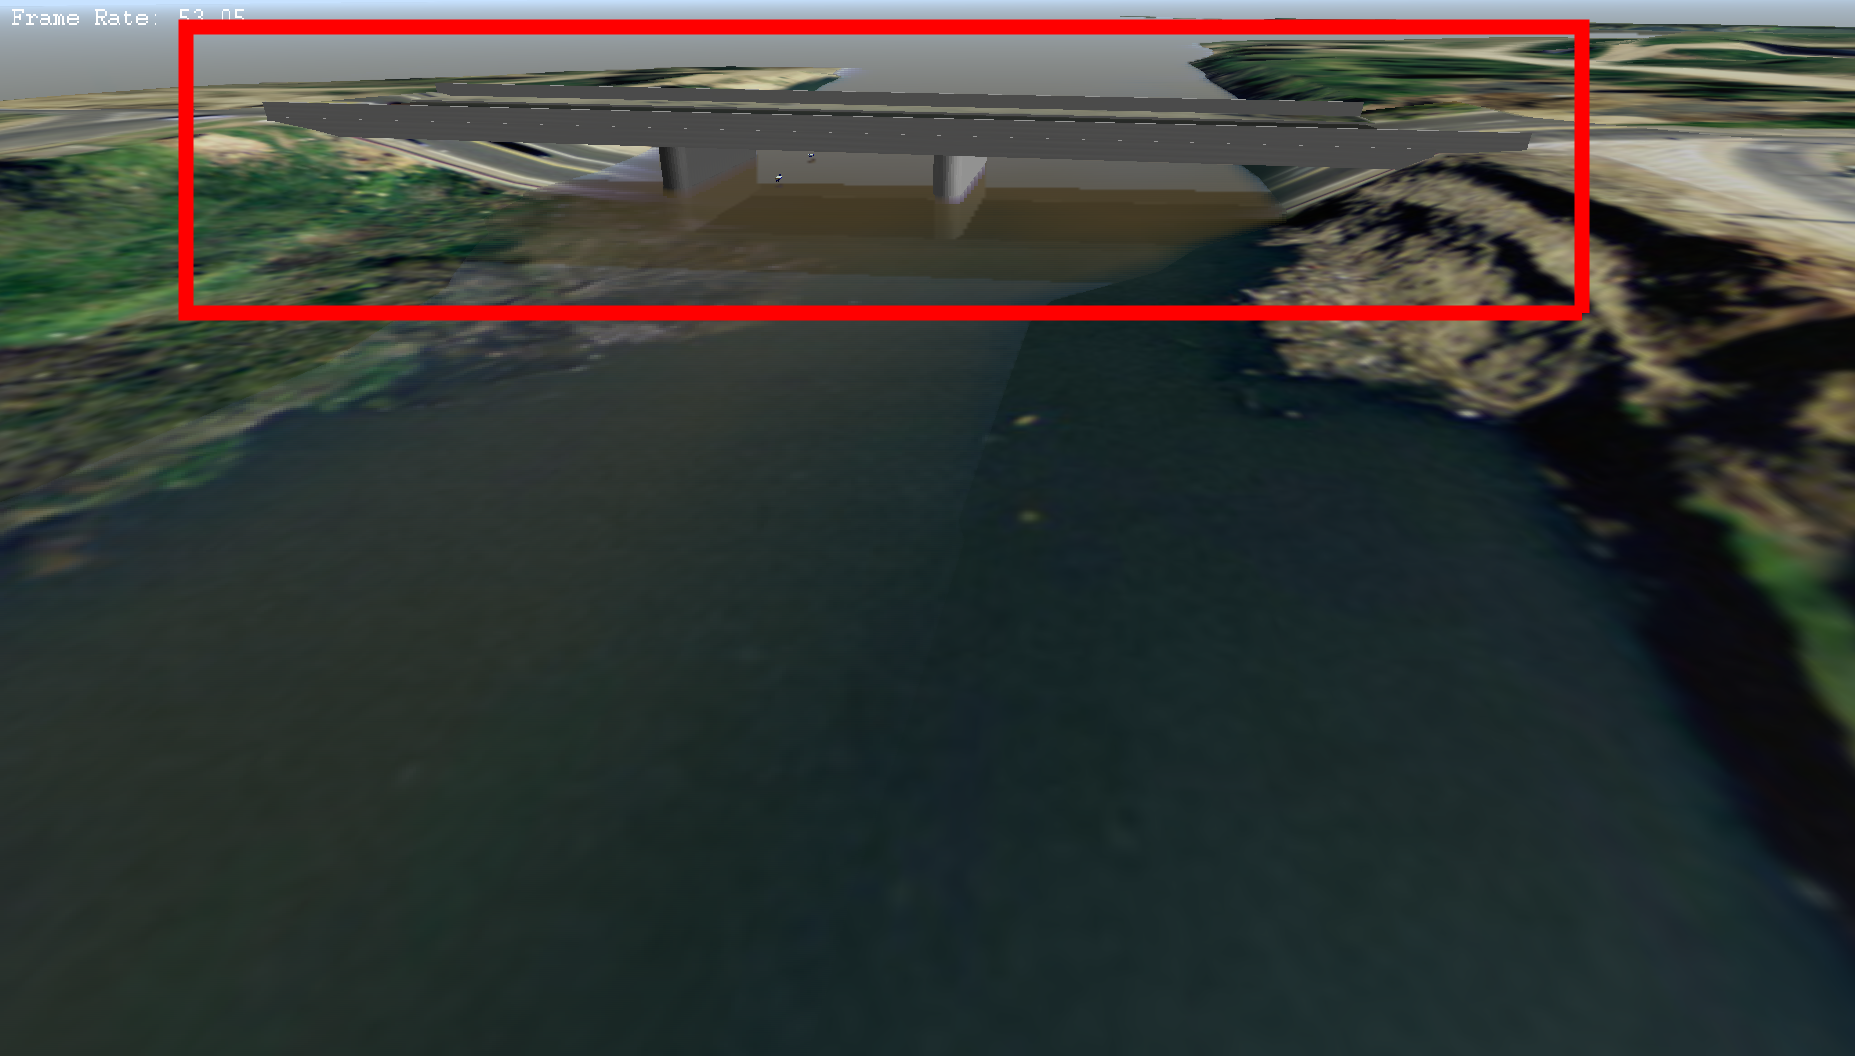
\includegraphics[scale=0.11]{figs/Chap5/simulation_diluvio_googleLocation2_2_roundedArea.png}
            \caption{Simulated version of Real World Location }
            \label{fig:simulation_diluvio_googleLocation2_2_roundedArea}
        \end{subfigure}
    
    \caption{Real world region and its simulated version}
    \label{fig:simulation_diluvio_googleLocation2_roundedArea}
    \end{figure}
    
    
    \begin{figure}[H]
        \centering
        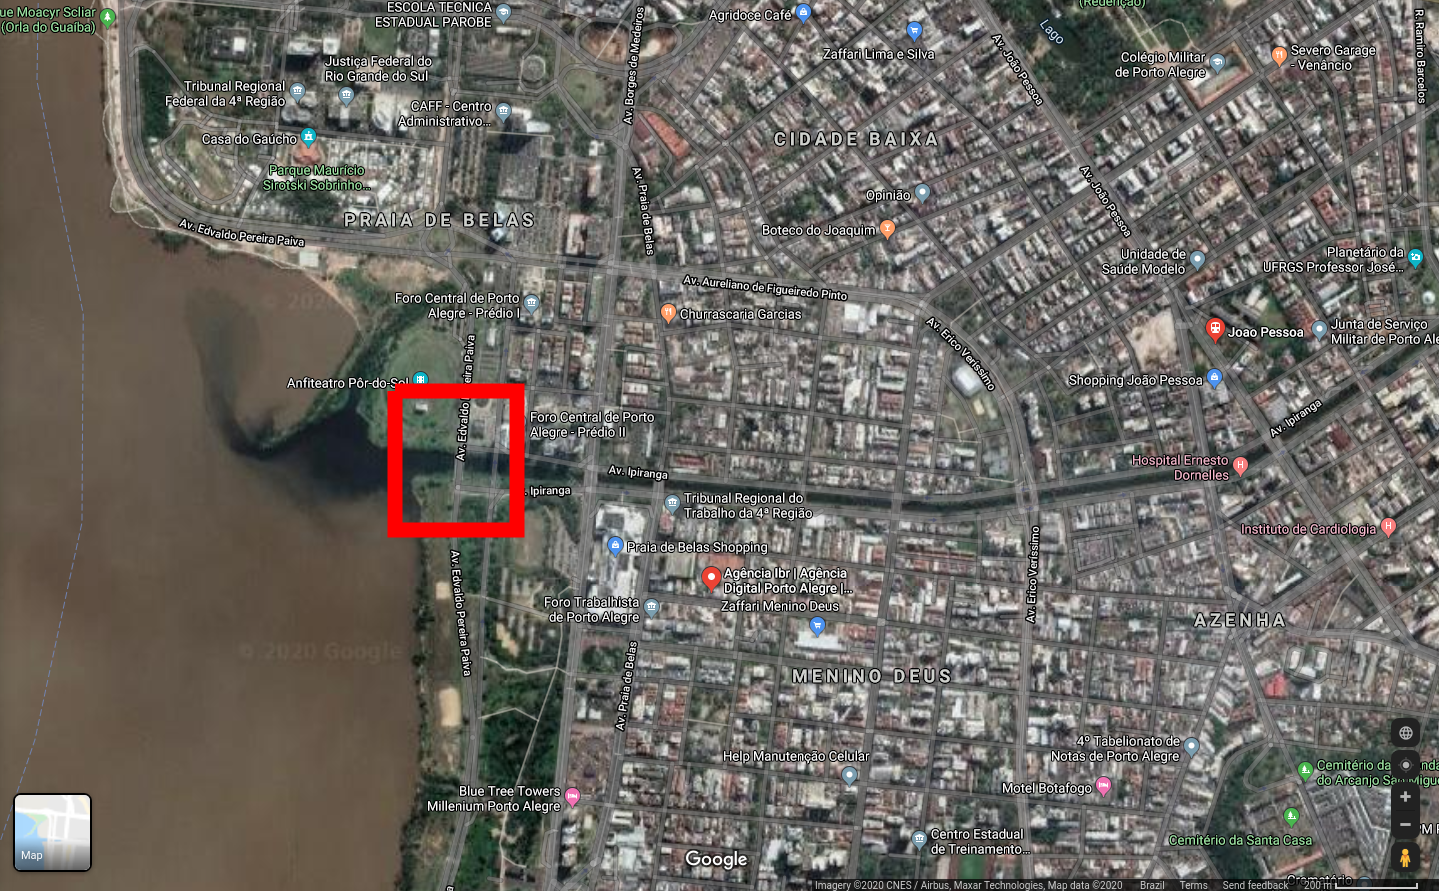
\includegraphics[scale=0.3]{figs/Chap5/simulation_diluvio_googleLocation_roundedArea.png}
        \caption{Real-world location of the area we choose for evaluation of our system. This is a potential place for real-world trials of our system, once it is near our laboratory, so we evaluate the behavior of our system on it. Google maps location (-30.047258°, -51.232660°), Av. Edvaldo Pereira Paiva, 1970 - Praia de Belas - Porto Alegre - RS - Brazil}
        \label{fig:simulation_diluvio_googleLocation_roundedArea}
    \end{figure}
    % \todo{cite some characteristics of the region}
    
    \begin{figure}[H]
    \centering
    
        \begin{subfigure}[b]{0.495\textwidth}
            \centering
            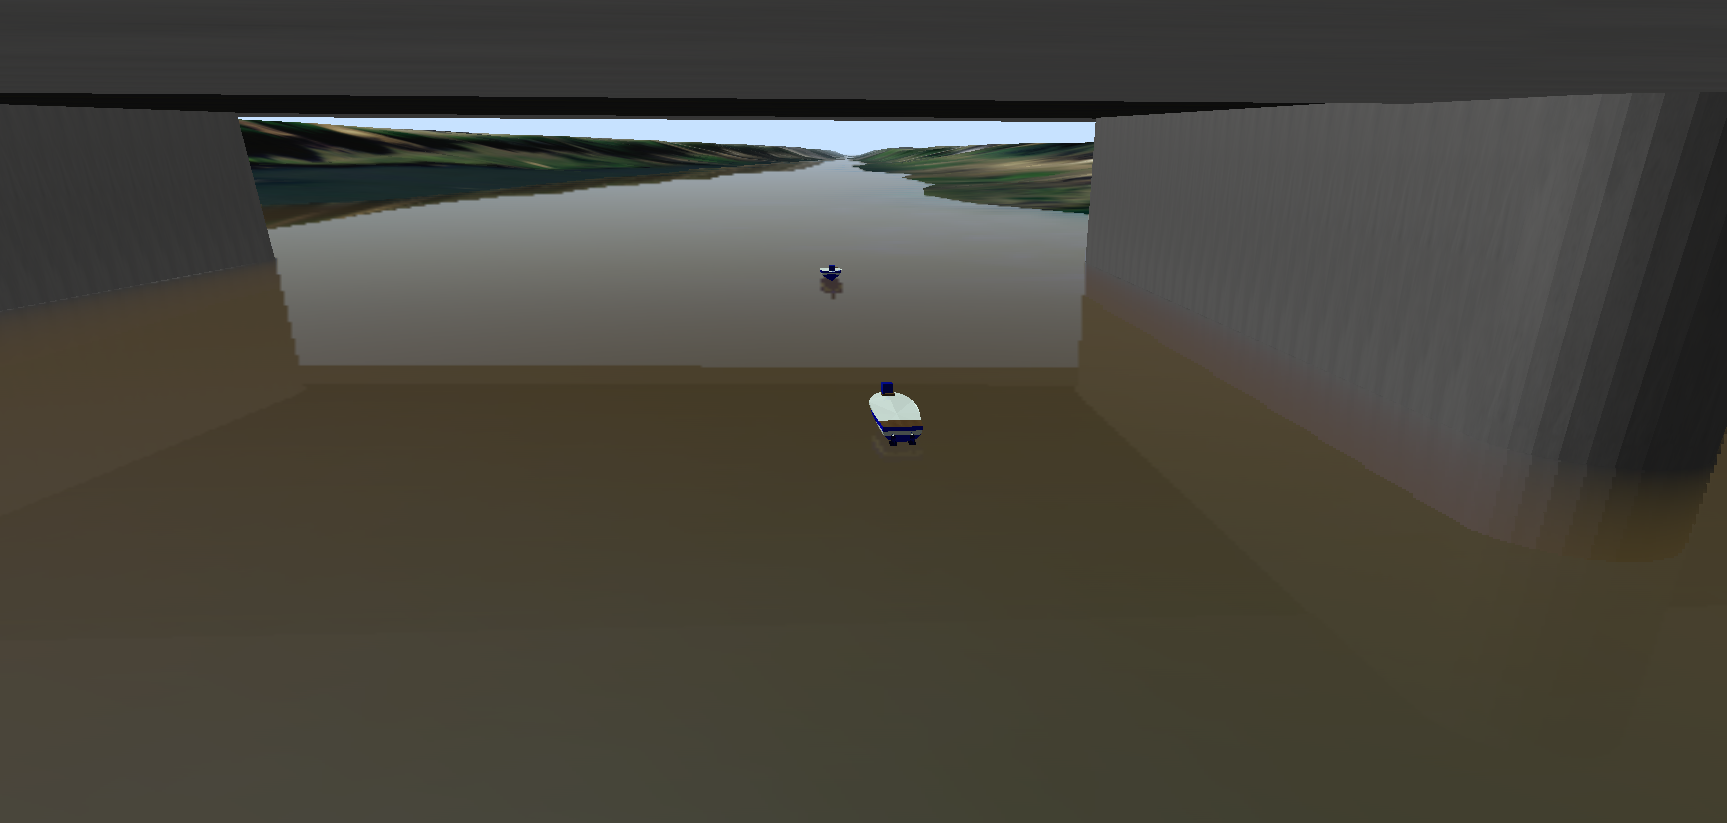
\includegraphics[width=\textwidth]{figs/Chap5/simulation_uwsim_headon_starting_pos.png}
            \caption{Head On}
            \label{fig:simulation_uwsim_headon_starting_pos}
        \end{subfigure}
        \begin{subfigure}[b]{0.495\textwidth}
            \centering
            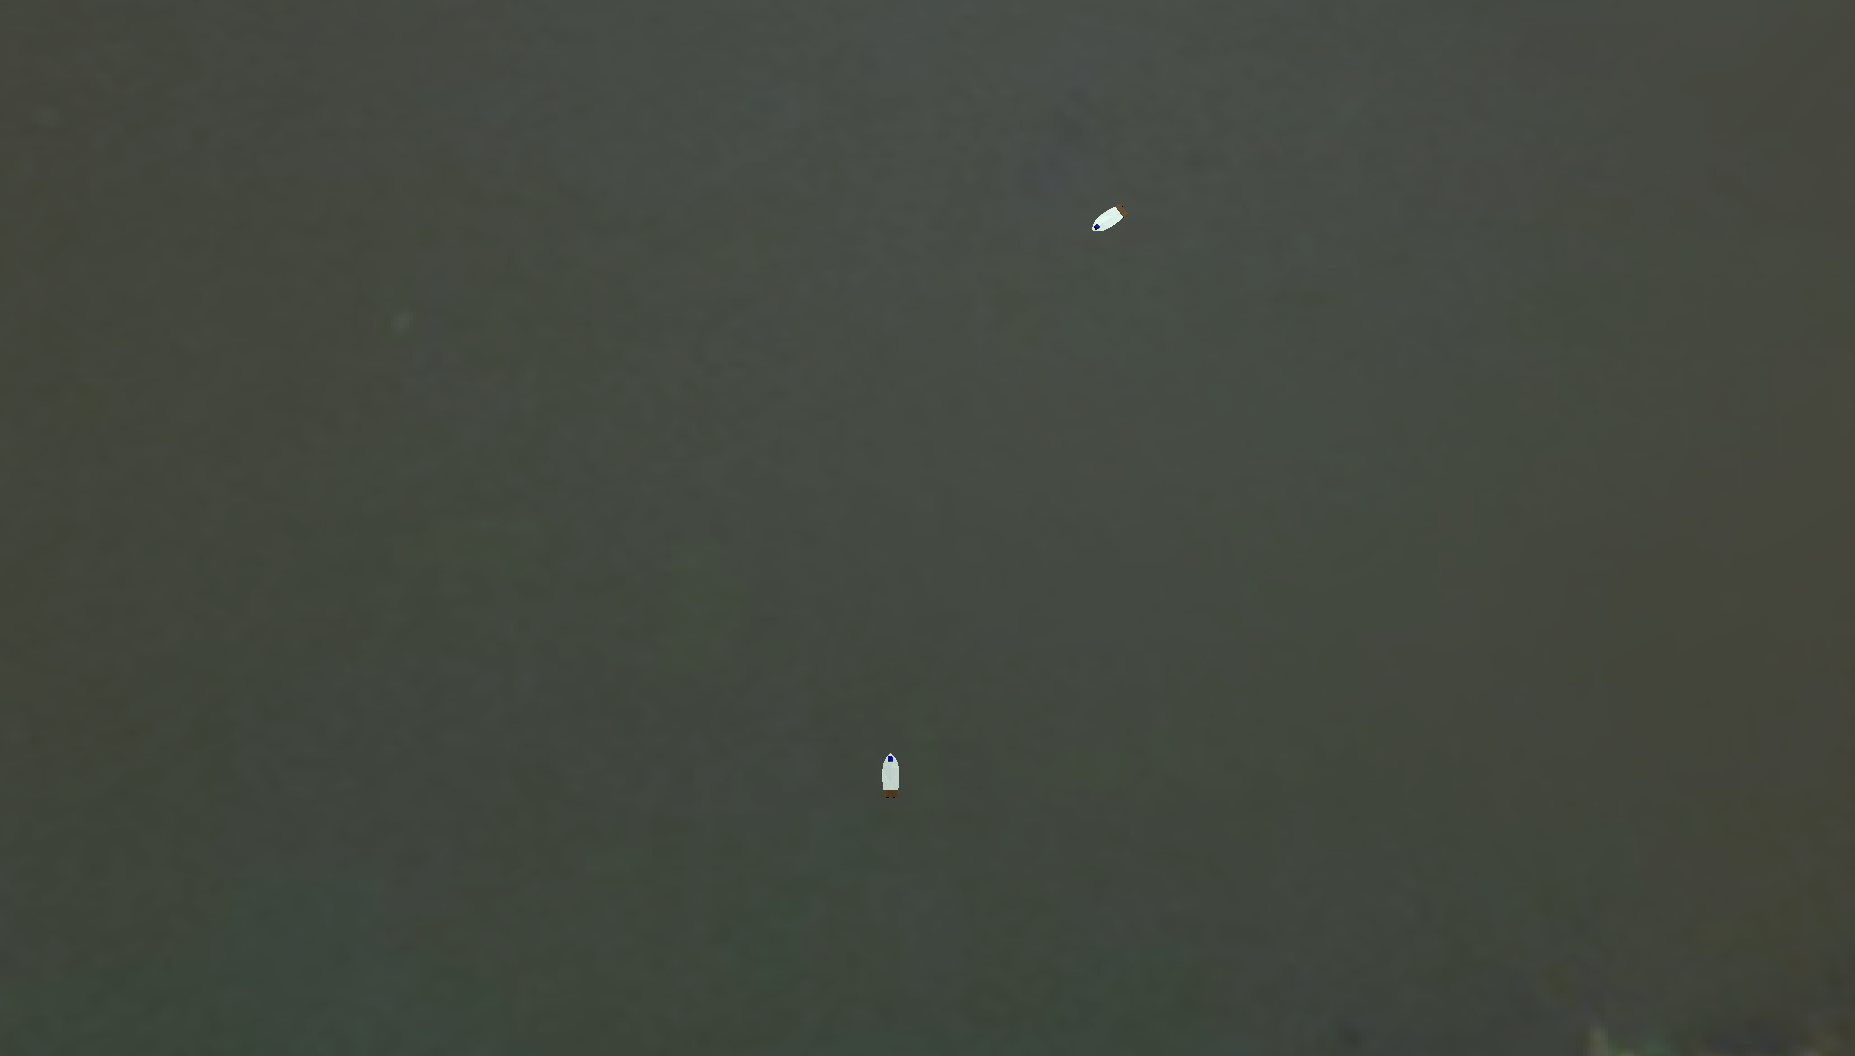
\includegraphics[width=\textwidth]{figs/Chap5/simulation_uwsim_crossingright_starting_pos.png}
            \caption{Crossing from Right}
            \label{fig:simulation_uwsim_crossingright_starting_pos}
        \end{subfigure}
        
        \begin{subfigure}[b]{0.495\textwidth}
            \centering
            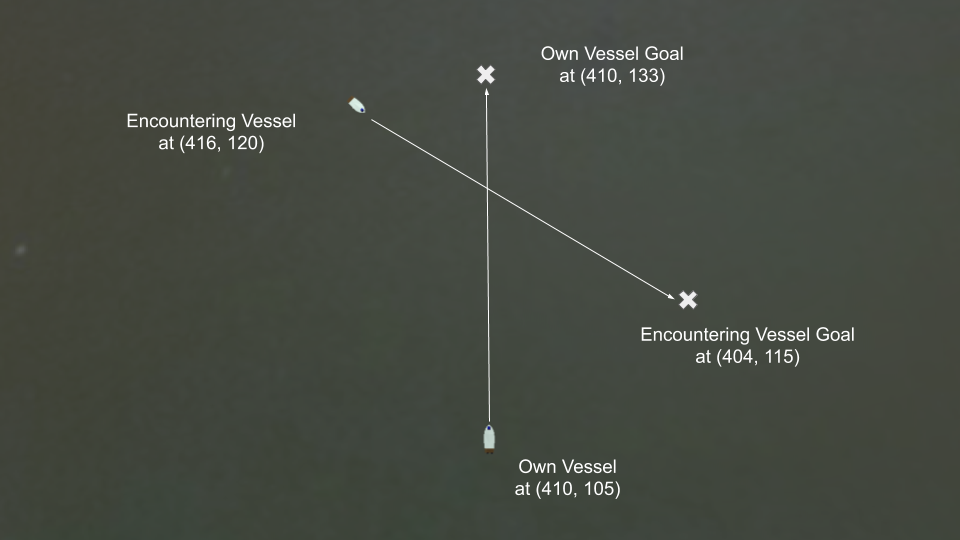
\includegraphics[width=\textwidth]{figs/Chap5/simulation_uwsim_crossingleft_starting_pos.png}
            \caption{Crossing from Left}
            \label{fig:simulation_uwsim_crossingleft_starting_pos}
        \end{subfigure}
        \begin{subfigure}[b]{0.495\textwidth}
            \centering
            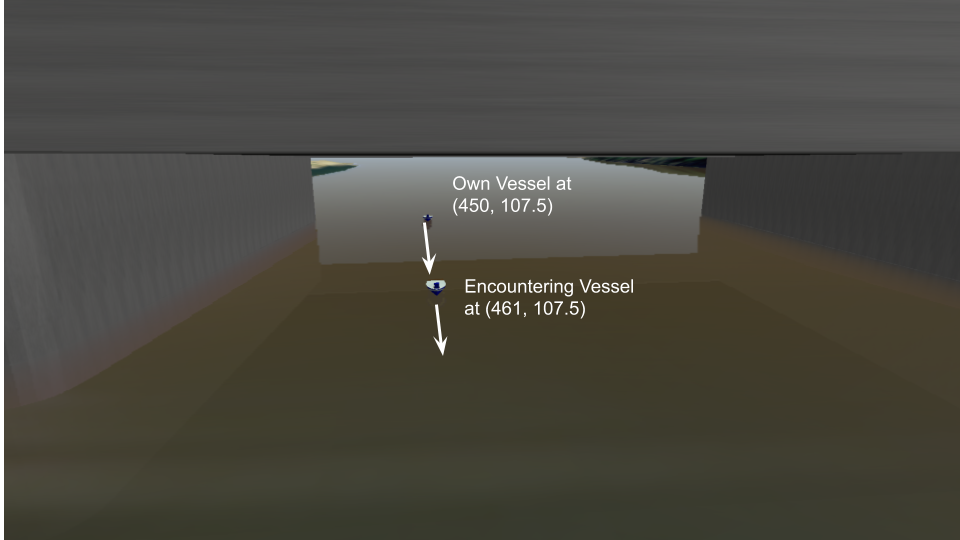
\includegraphics[width=\textwidth]{figs/Chap5/simulation_uwsim_overtake_starting_pos.png}
            \caption{Overtaking}
            \label{fig:simulation_uwsim_overtake_starting_pos}
        \end{subfigure}
    
    \caption{Encounter scenarios for evaluation. Scenarios adapted from ~\cite{Huang2019Generalized}.}
    \label{fig:simulation_uwsim_encounters}
    \end{figure}

%AMA a figura dos barcos esta muito pequena. veja como fica na versao impressa. acho q vc vai ter q pelo menos desenhar uma flecha p indicar a direcao dos barcos.
%DJ:

    \begin{center}
        \savebox{\mytablebox}{\begin{tabular}{cccc}
        
        \toprule[3pt]
        \multicolumn{4}{c}{\textbf{\ac{OV}}} \\
        % \multicolumn{3}{c}{\textbf{\ac{OV}}} \\
        \midrule
        \textbf{Encounter Type} & \textbf{Initial Pose (m, m, º)} & \textbf{Target Position} &  \textbf{Max. Speed (m/s)}\\
        \midrule
        Head On &  (450, 107.5, 0)  &   (480, 107.5)  &  0.4 \\
        Crossing Right &  (410, 105, 90)  &  (410, 133)  &  0.86  \\
        Crossing Left &  (410, 105, 90)  & (410, 133)   &  0.29  \\
        Overtaking &  (450, 107.5, 0)  &  (600, 107.5) &  0.5 \\
        \bottomrule
        
        \end{tabular}}
        \settowidth{\mytablewidth}{\usebox{\mytablebox}}
        \begin{minipage}{\mytablewidth}
        \captionof{table}{Encounter Scenarios Configuration - \ac{OV}}
        \label{tab:simulation_scenarios_configuration_own_vessel}
        \usebox{\mytablebox}
        \end{minipage}

    \end{center}
    
    \begin{center}
        % \savebox{\mytablebox}{\begin{tabular}{cccc}
        \savebox{\mytablebox}{\begin{tabular}{cccc}
        
        \toprule[3pt]
        \multicolumn{4}{c}{\textbf{\ac{EV}}} \\
        % \multicolumn{3}{c}{\textbf{\ac{EV}}} \\
        \midrule
        \textbf{Encounter Type} & \textbf{Initial Pose (m, m, º)} & \textbf{Target Position} & \textbf{Max. Speed (m/s)}\\
        \midrule
        Head On &  (461, 107.5, 180)  &   (350, 107)  &  0.4 \\
        Crossing Right &  (416, 120, 215)  &  (404, 115)  &  0.86  \\
        Crossing Left &  (404, 105, 315)  & (416, 115)  &  0.29  \\
        Overtaking &  (461, 107.5, 0)  &  (600, 107)  &  0.5 \\
        \bottomrule
        
        \end{tabular}}
        \settowidth{\mytablewidth}{\usebox{\mytablebox}}
        \begin{minipage}{\mytablewidth}
        \captionof{table}{Encounter Scenarios Configuration - \ac{EV}}
        \label{tab:simulation_scenarios_configuration_encountering_vessel}
        \usebox{\mytablebox}
        \end{minipage}

    \end{center}

%AMA a apresentacao da tabela está realmente feia ! Latex tem formatos bem legais. Sugiro melhorar esse aspecto. Tb sugiro fortemente colocar na fig anterior o local do initial pose, destination, e trajetoria. Acho q deve trocar Waypoint por destination ou target position.
%DJ: Done

    % Grammarlly: 100/100
    % Agrawal \etal ~\cite{Agrawal2015COLREGS} evaluate theirs A* approach in a 100mx100m grid with a resolution of 1:1, resulting in a search space of 10000 cells, we built our scenarios respecting the same proportionality. In all scenarios, our \ac{USV} plan in a 20mx20m grid with 1:0.2 resolution, resulting in a search space of 10000 cells, see Figure \ref{fig:rviz_local_costmap}. The choice of 20mx20m dimension is related to real limitations of the range and reliability on laser sensors, the RPLIDAR A3 laser~\cite{RPLidarA3} model, for example, is reliably capable of detection in 25 meters distance range.
    
    \section{Experiments Results}

        %%%%%%%%%%%%%%%%%%%%%%%%%%%%%%%%%%%%%%
        %% Intro to Experiments Results
        %
        %% Grammarlly: 93/100
        %% v2.0
        %%%%%%%%%%%%%%%%%%%%%%%%%%%%%%%%%%%%%%
        We qualitatively evaluated the behavior of our method in two different configurations. In the first configuration, we compare the behavior of the system with and without \ac{ATC}, and in the second configuration, we compare the behavior of our system with \ac{ATC} under the influence of wind and without the influence of wind. We executed both scenarios for four types of possible encounters between two vessels. For quantitative evaluation of each scenario, we measured the computation time of every execution of our path planner, average sustained speed, and minimal distance maintained between the vessels, as well as we evaluated whether the collision avoidance was successful or not. In Table \ref{tab:results} we summarize the collected results.

        %%%%%%%%%%%%%%%%%%%%%%%%%%%%%%%%%%%%%%
        %% Head-On w vs wo \ac{ATC}
        %
        %% Grammarlly: 99/100
        %%%%%%%%%%%%%%%%%%%%%%%%%%%%%%%%%%%%%%
        Figure \ref{fig:plot_ho_w_vs_wo} presents, comparatively, the final trajectory of two vessels in two executions of the same head-on scenario. For the \ac{OV}, the performed trajectory is guided by our local guidance system, and \ac{EV} from its start position must go to a goal ahead. In the "\ac{ATC} case" execution, our system is fully functional, in the "no \ac{ATC}" execution we removed the ability of the planning system to generate virtual obstacles, which is the core of the \ac{ATC} method and partially responsible for the COLREGS-Compliant path planning. In both runs, in the time interval from t0 until just before t1 \ac{OV} takes off in the northeast direction, due to a static obstacle located from (450, 104) to (460, 104).
        
        Until t1, \ac{OV} tends to distance itself from the static obstacle, at t1 for both executions of the scenario, \ac{EV} becomes noticeable at the \ac{OV} local cost map. From t1 \ac{OV} react differently to each encounter. We observe that even with the existence of a static obstacle to the south in its proximity, \ac{OV} in \ac{ATC} case decides to avoid the encounter with the other vessel moving to its starboard side, featuring a COLREGS-Compliant behavior. \ac{OV} in "no \ac{ATC}" case, influenced only by the existence of an obstacle in the south and the encounter with \ac{EV}, defines a not COLREGS-compliant path.
        
        % \begin{figure}[H]
        % \centering
        
        %     \begin{subfigure}[b]{0.45\textwidth}
        %         \centering
        %         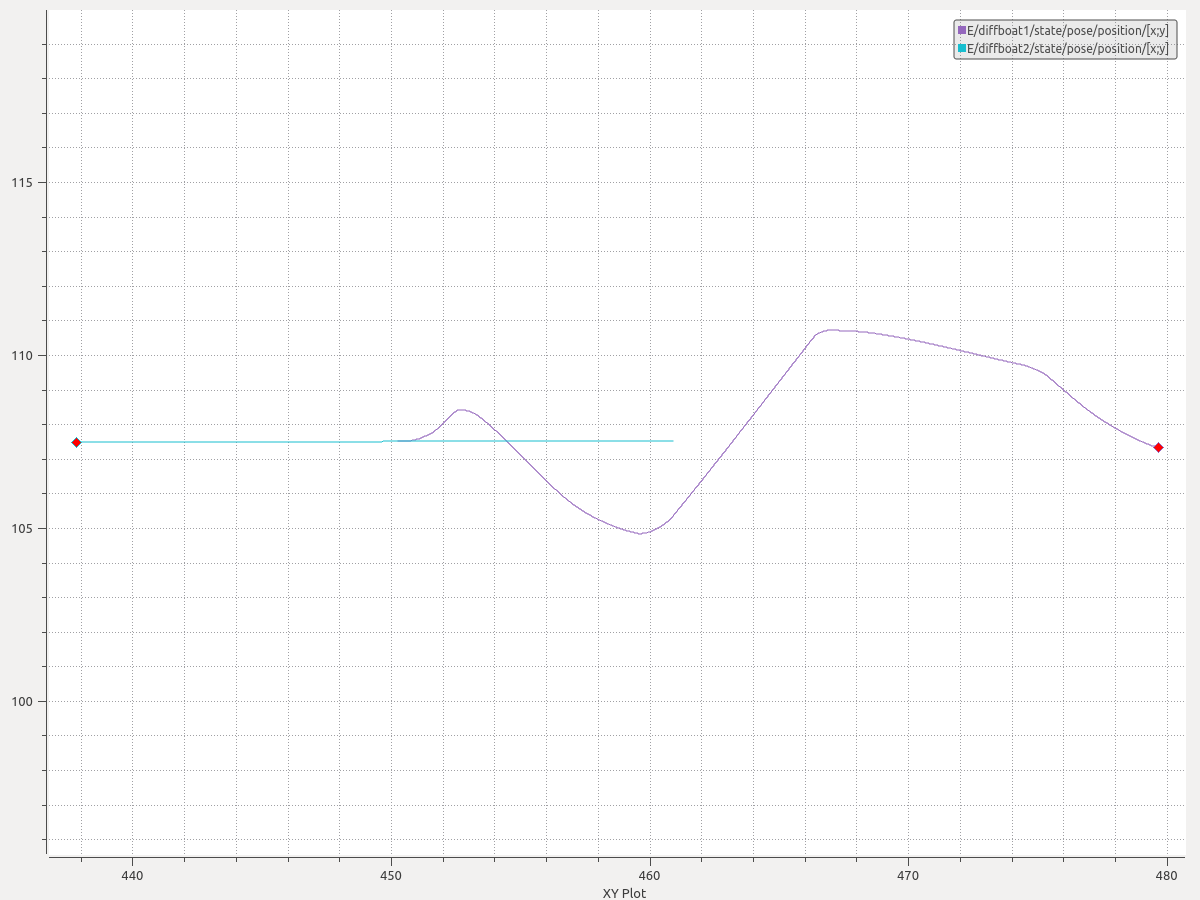
\includegraphics[width=\textwidth]{figs/Chap5/plot_headOn_E.png}
        %         \caption{With \ac{\ac{ATC}}}
        %         \label{fig:plot_headOn_E}
        %     \end{subfigure}
        %     \begin{subfigure}[b]{0.45\textwidth}
        %         \centering
        %         \includegraphics[width=\textwidth]{figs/Chap5/plot_no\ac{ATC}_headOn_E.png}
        %         \caption{Without \ac{\ac{ATC}}}
        %         \label{fig:plot_no\ac{ATC}_headOn_E}
        %     \end{subfigure}
            
        %     \begin{subfigure}[b]{0.45\textwidth}
        %         \centering
        %         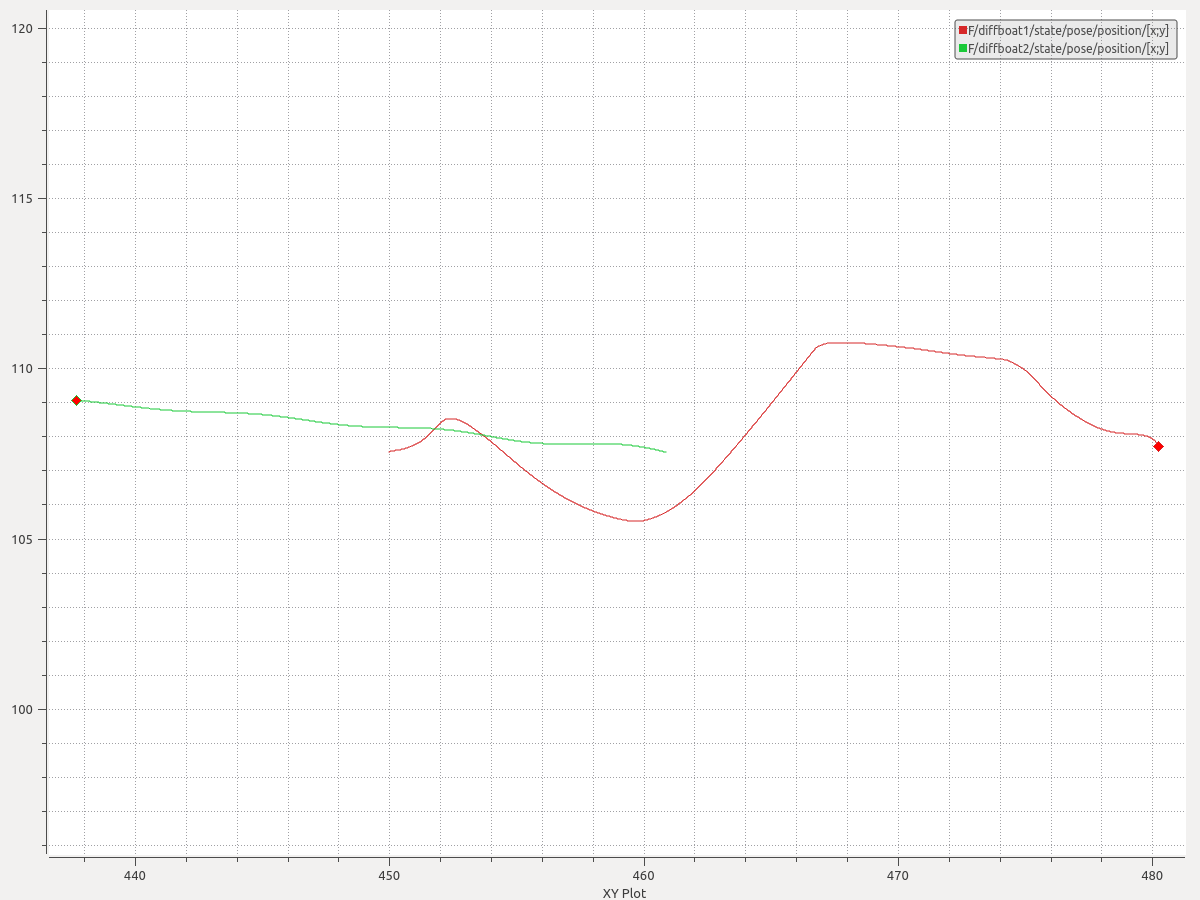
\includegraphics[width=\textwidth]{figs/Chap5/plot_headOn_Wind_E.png}
        %         \caption{With \ac{\ac{ATC}} and Wind}
        %         \label{fig:plot_headOn_Wind_E}
        %     \end{subfigure}
        %     % \begin{subfigure}[b]{0.45\textwidth}
        %     %     \centering
        %     %     \includegraphics[width=\textwidth]{figs/Chap5/plot_Overtaking_Wind_BAD_E.png}
        %     %     \caption{\ac{\ac{ATC}} and Bad Wind}
        %     %     \label{fig:plot_headOn_Wind__BAD_E}
        %     % \end{subfigure}
        
        % \caption{DESCRIÇÂO DOS GRAFICOS AQUI: }
        % \label{fig:headOn_E}
        % \end{figure}
%AMA a legenda dass trajetorias esta ilegivel. ou vc aumenta ate ficar legivel ou remove dali. se remover, vc pode descrever o significado das cores na legenda.
%AMA do jeito q está, nao eh facil comparar um grafico c o outro. seria MUITO melhor se vc conseguir colocar dois plots juntos. por exemplo, with \ac{ATC} e wo/ \ac{ATC}. with \ac{ATC} e with \ac{ATC} + wind. Nao junta os 3 pois acho q vai poluir demais.
% AMA a legenda dos eixos tb nao deve estar legivel p impressao. aumente o texto dos nros.
%AMA o ponto vermelho eh o ponto inicial ou final. deixar isso claro na legenda
%AMA qnd tiver vento, anota na figura a dirececao e velocidade tb.

        \begin{figure}[H]
            \centering
            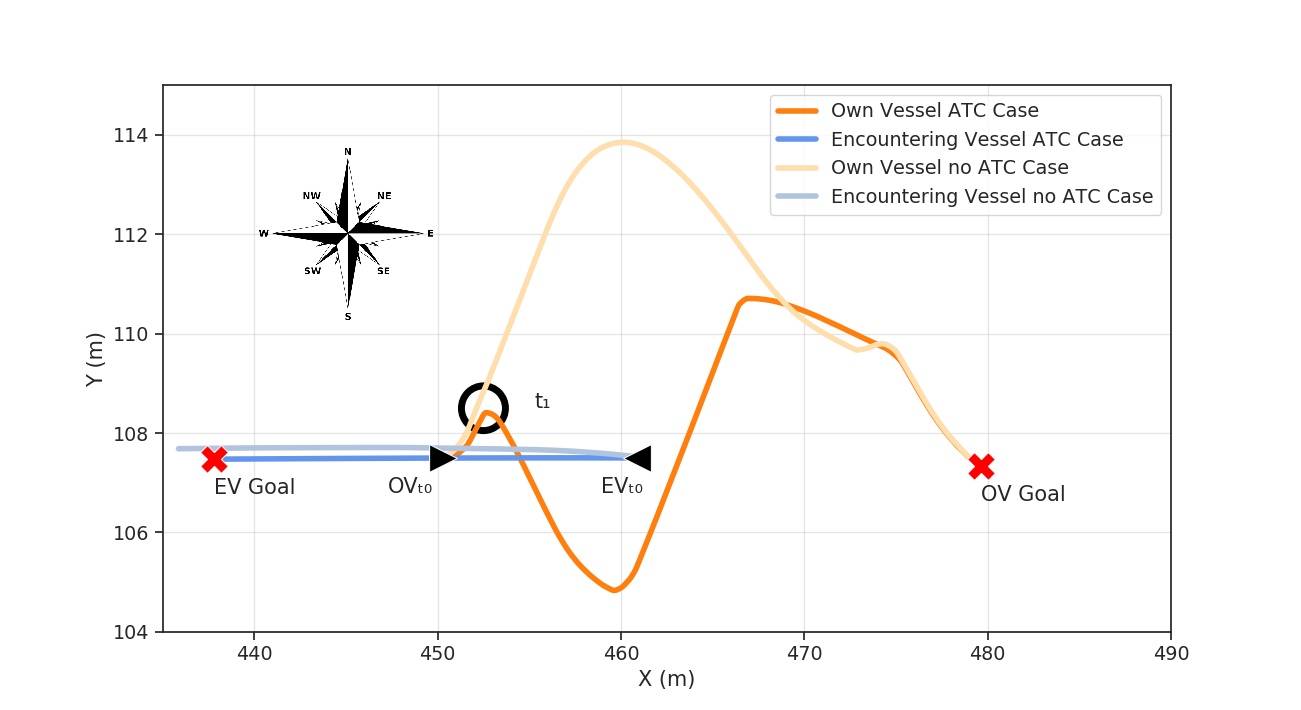
\includegraphics[width=\textwidth]{figs/Chap5/plot_ho_w_vs_wo.png}
            \caption{Vessels trajectories comparison between \ac{ATC} case versus no \ac{ATC} in a head-on encounter scenario. Start position for \ac{OV} and \ac{EV} are marked with ">" and "<", while their goals are marked with "x". Here we can observe that our \ac{ATC} A* method implied COLREGS compliance, once in a detection of another vessel ($t_1$) it generated a COLREGS-Compliant path, avoiding collision going to its starboard side.}
            \label{fig:plot_ho_w_vs_wo}
        \end{figure}
        
        %%%%%%%%%%%%%%%%%%%%%%%%%%%%%%%%%%%%%%
        %% Head-On w vs wo \ac{ATC} Computational Time
        %
        %% Grammarlly: 99/100
        %%%%%%%%%%%%%%%%%%%%%%%%%%%%%%%%%%%%%%
        Figure \ref{fig:plot_ho_w_vs_wo_CT} shows the computational time measured in seconds in a time series. Our COLREGS-Compliant \ac{ATC} A* method had a peek cost of 0.369s for path generation for this head-on scenario. As we can see, both \ac{ATC} case and no \ac{ATC} have similar computational cost curves. This happens because most of the computational cost of our path planning method is related to our A* implementation. The \ac{ATC} method alone has low computational consumption since it cost in the worst case in filling an area lxm, with l equals to \ac{OV}'s length and m equals to half of cost map greater dimension, that is O(n²);
        \begin{figure}[H]
            \centering
            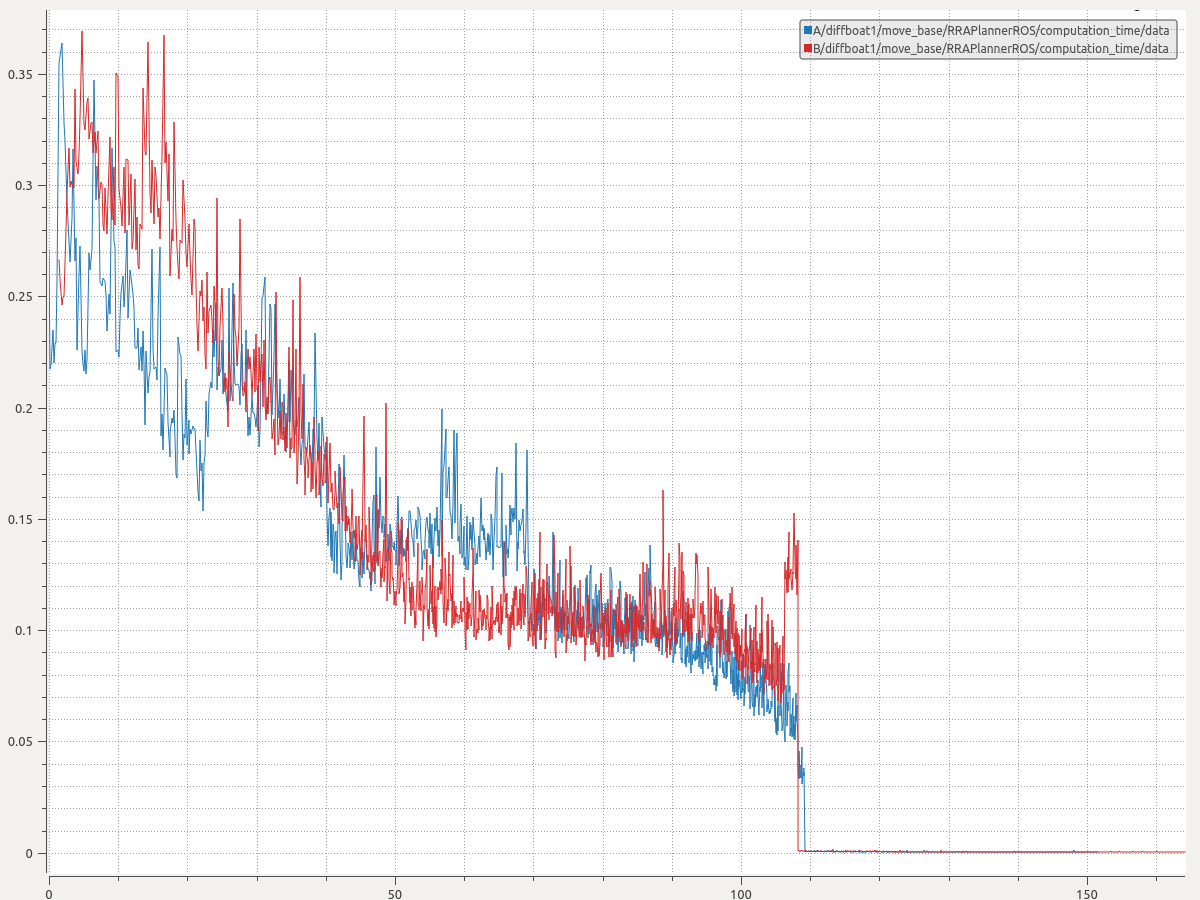
\includegraphics[width=\textwidth]{figs/Chap5/plot_ho_w_vs_wo_CT.png}
            \caption{Computational time comparison between \ac{ATC} case versus no \ac{ATC} in a head-on encounter during time series. The system achieves a peak cost of around 0.364s using \ac{ATC} and around 0.369 without \ac{ATC}. This happens due to an intrinsic characteristic of our A* method. At $t_1$ \ac{EV} appears in the limit of \ac{OV} local cost map in a conflicting position with local map A* goal. In this situation, the planning system searches for the nearest free position and define a path to it. After some time, \ac{EV} is not anymore in a conflicting position, and the computational time reduces dramatically. Due to this behavior, our system presents a low average execution time around 0.074s when compared to the maximum computational time.}
            \label{fig:plot_ho_w_vs_wo_CT}
        \end{figure}
        
        %%%%%%%%%%%%%%%%%%%%%%%%%%%%%%%%%%%%%%
        %% Head-On w vs wo Wind
        %
        %% Grammarlly: 99/100
        %%%%%%%%%%%%%%%%%%%%%%%%%%%%%%%%%%%%%%
        In Figure \ref{fig:plot_ho_w_vs_wind} we compare final trajectories for same head-on scenario described in \ref{tab:simulation_scenarios_configuration_own_vessel} for two executions of the simulation with different wind influence, in both executions contain \ac{ATC} A*. No wind case shows the behavior of the \ac{OV} being influenced by no wind. Wind case shows the trajectory of the vessel \ac{OV} being influenced by the wind with northeast direction and intensity of 0.2 m/s, indicated by an arrow. We can see the change in the trajectory of \ac{OV} and that it still to maintain COLREGS-compliance. \ac{EV} response to the wind is related to the standard control system used; in this work, we do not evaluate the limitations of this system.
        \begin{figure}[H]
            \centering
            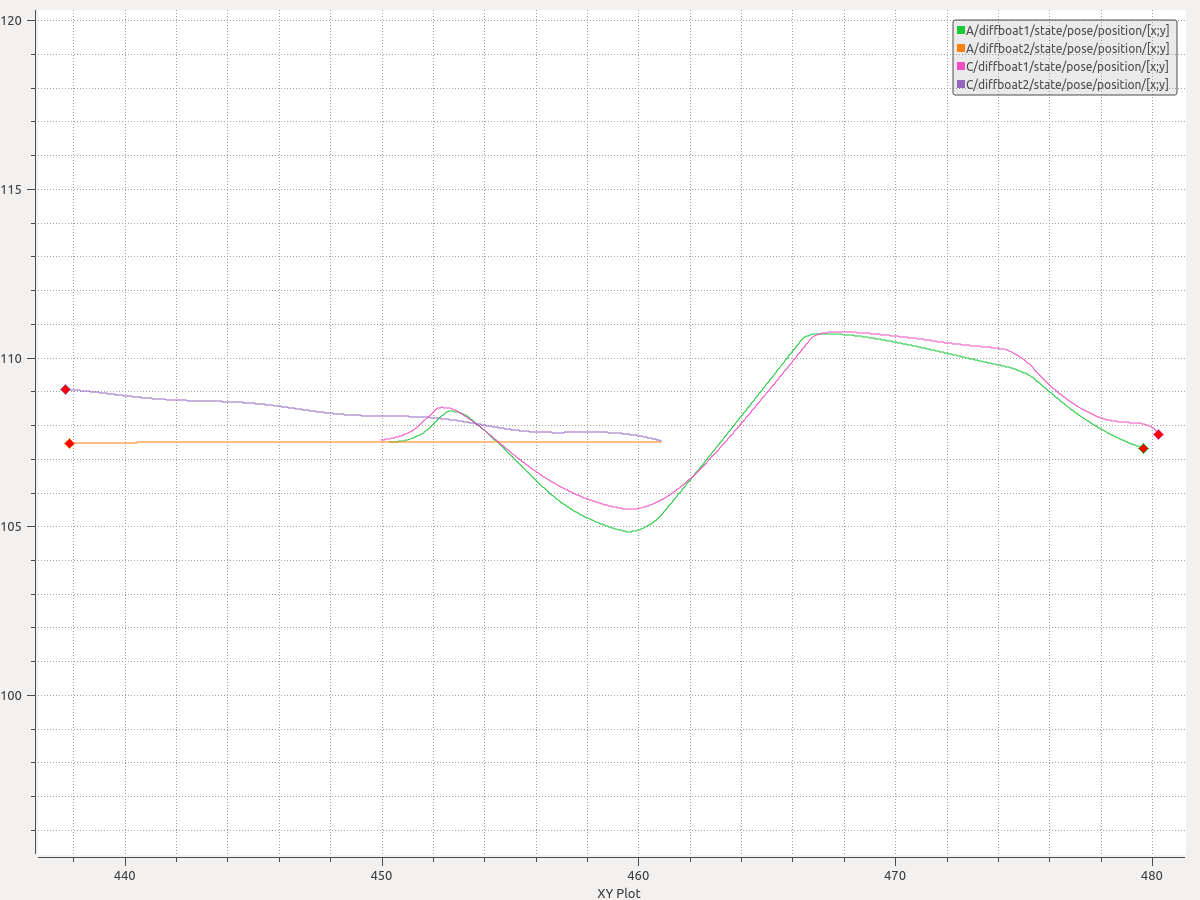
\includegraphics[width=\textwidth]{figs/Chap5/plot_ho_w_vs_wind.png}
            \caption{Comparison between the trajectories of the vessels in Wind case and no Wind case in a head-on encounter scenario, both cases use \ac{ATC} A*. Start position for \ac{OV} and \ac{EV} are marked with ">" and "<", while their goals are marked with "x". For the Wind case, the direction of the wind is northeast, represented by an arrow. We can observe that our \ac{ATC} A* kept implying COLREGS compliance even under the influence of wind in this scenario.}
            \label{fig:plot_ho_w_vs_wind}
        \end{figure}
        
        %%%%%%%%%%%%%%%%%%%%%%%%%%%%%%%%%%%%%%
        %% Head-On w vs wo Wind Computational Time
        %
        %% Grammarlly: 100/100
        %%%%%%%%%%%%%%%%%%%%%%%%%%%%%%%%%%%%%%
        Figure \ref{fig:plot_ho_w_vs_wind_CT} shows the computational time measured in seconds in a time series for wind and no wind cases. We observe that the computational time keep similar and does not seems to be related to the imposed wind influence for this simulation.
        \begin{figure}[H]
            \centering
            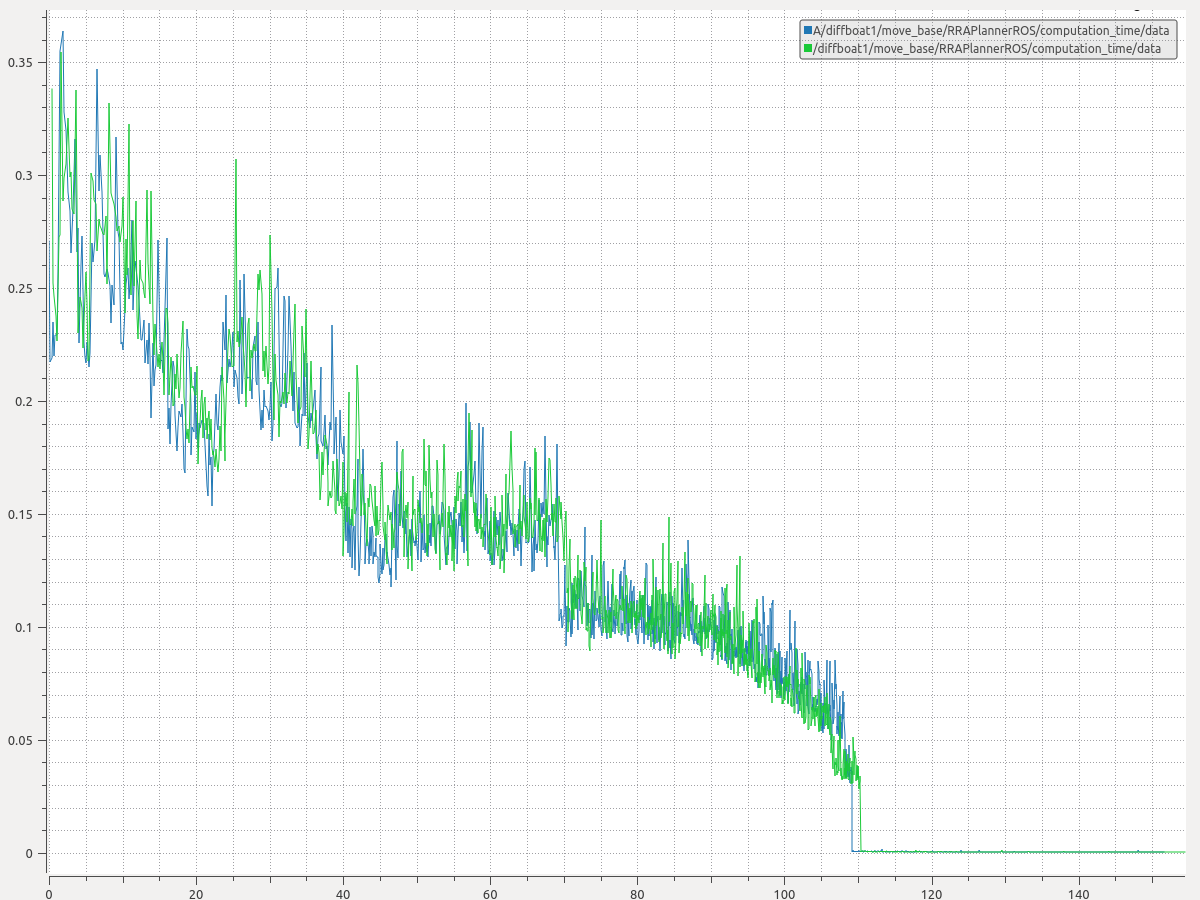
\includegraphics[width=\textwidth]{figs/Chap5/plot_ho_w_vs_wind_CT.png}
            \caption{Computational time comparison between Wind case versus no Wind in a head-on encounter.}
            \label{fig:plot_ho_w_vs_wind_CT}
        \end{figure}
        
        %%%%%%%%%%%%%%%%%%%%%%%%%%%%%%%%%%%%%%
        %% Crossing Right w vs wo \ac{ATC}. w vs wo Wind
        %
        %% Grammarlly: 100/100
        %%%%%%%%%%%%%%%%%%%%%%%%%%%%%%%%%%%%%%
        In Figure \ref{fig:plots_cr}, we present the behavior of our system when \ac{OV} encounters another vessel coming from the right. In Figure \ref{fig:plot_cr_w_vs_wo} we show the comparison between trajectories with and without ATC and in Figure \ref{fig:plot_cr_w_vs_wo_CT} we can see computational time for each case. As we can see, our method implies COLREGS compliance when avoiding a collision.
        
        In Figure \ref{fig:plot_cr_w_vs_wind} we show the comparison between trajectories with and without wind influence and in Figure \ref{fig:plot_cr_w_vs_wind_CT} we can see computational time for each case. As we can see, once again, our method kept COLREGS-compliant even when disturbed by a maximum of 0.2 m/s wind.
        
        \begin{figure}[H]
        \centering
        
            \begin{subfigure}[b]{0.49\textwidth}
                \centering
                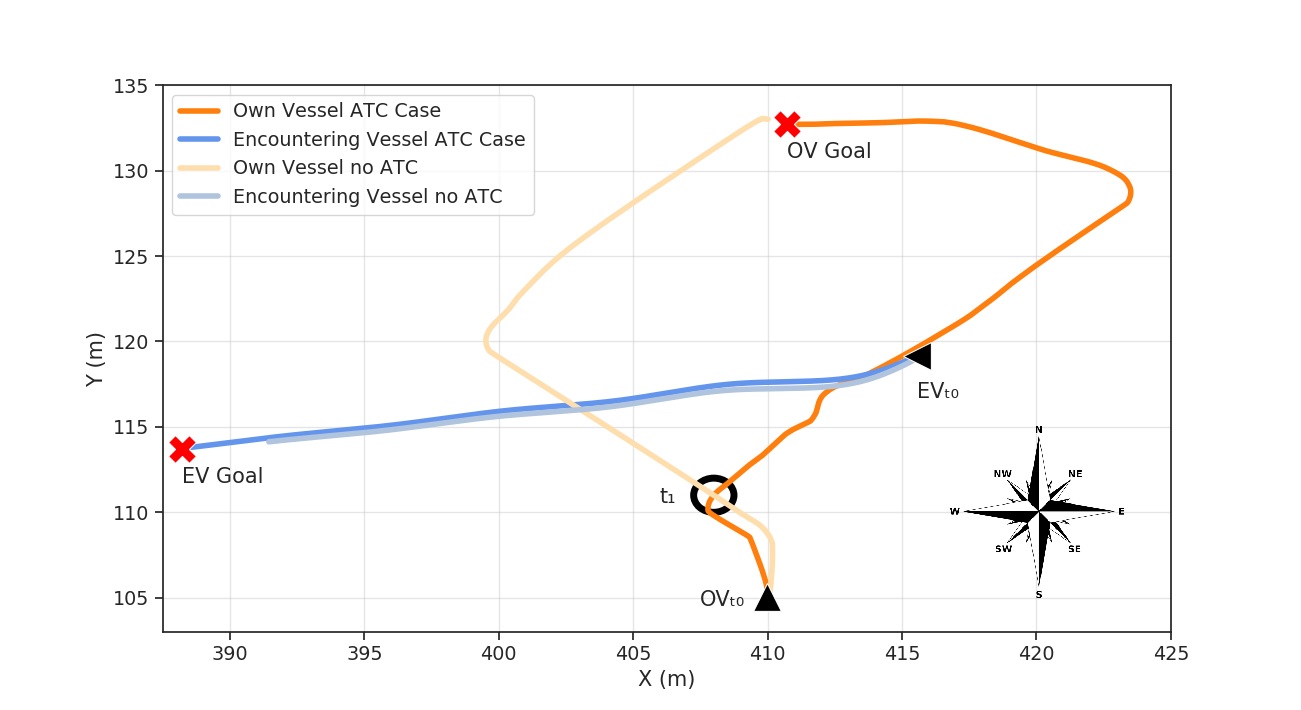
\includegraphics[width=\textwidth]{figs/Chap5/plot_cr_w_vs_wo.png}
                % \caption{Trajectory comparison between \ac{ATC} and no \ac{ATC} cases.}
                \caption{}
                \label{fig:plot_cr_w_vs_wo}
            \end{subfigure}
            \begin{subfigure}[b]{0.49\textwidth}
                \centering
                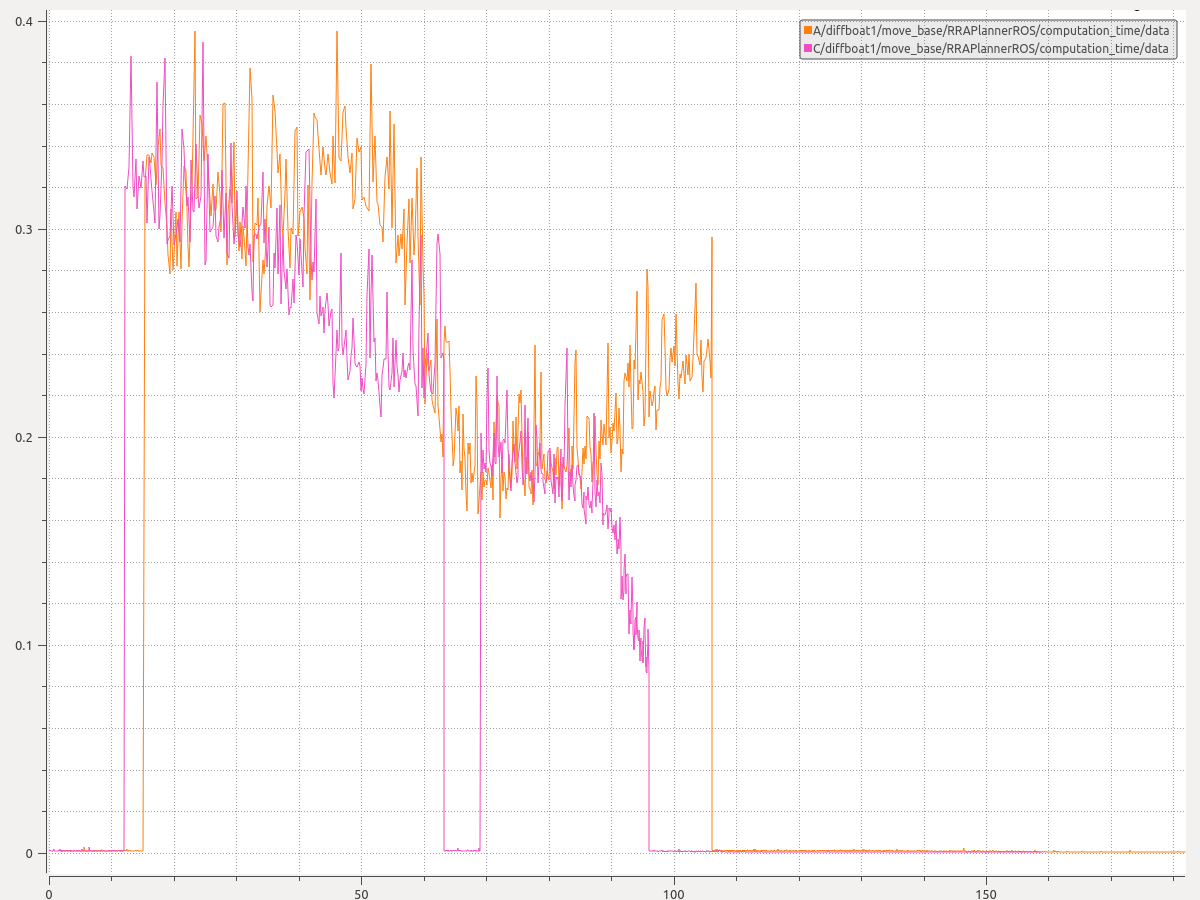
\includegraphics[width=\textwidth]{figs/Chap5/plot_cr_w_vs_wo_CT.png}
                % \caption{Computation Time. \ac{ATC} and no \ac{ATC} cases.}
                \caption{}
                \label{fig:plot_cr_w_vs_wo_CT}
            \end{subfigure}
            
            \begin{subfigure}[b]{0.49\textwidth}
                \centering
                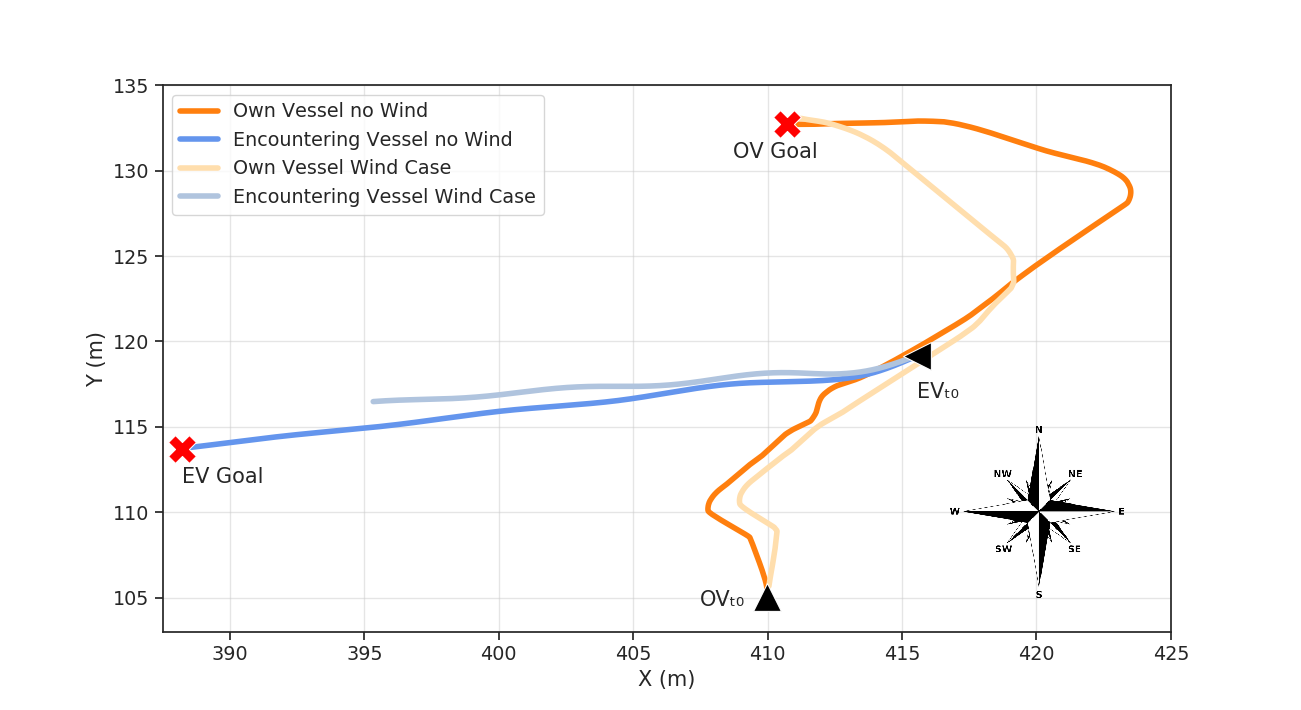
\includegraphics[width=\textwidth]{figs/Chap5/plot_cr_w_vs_wind.png}
                % \caption{Trajectory comparison between Wind and no Wind cases}
                \caption{}
                \label{fig:plot_cr_w_vs_wind}
            \end{subfigure}
            \begin{subfigure}[b]{0.49\textwidth}
                \centering
                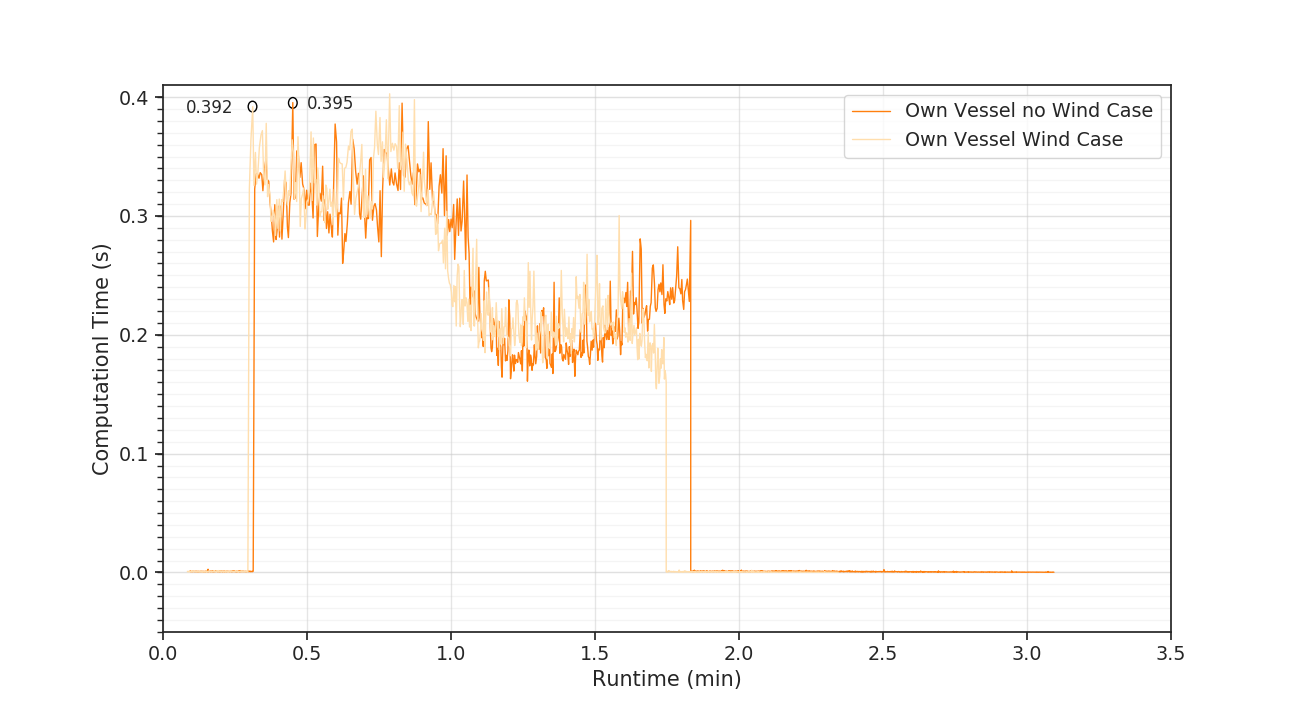
\includegraphics[width=\textwidth]{figs/Chap5/plot_cr_w_vs_wind_CT.png}
                % \caption{Computation Time. Wind and no Wind cases.}
                \caption{}
                \label{fig:plot_cr_w_vs_wind_CT}
            \end{subfigure}
        
        \caption{Crossing Right Encounter Scenario. Comparison between \ac{ATC} and no \ac{ATC}, and Wind cases.}
        \label{fig:plots_cr}
        \end{figure}
        
        %%%%%%%%%%%%%%%%%%%%%%%%%%%%%%%%%%%%%%
        %% Overtaking w vs wo \ac{ATC}. w vs wo Wind
        %
        %% Grammarlly: ?/100
        %%%%%%%%%%%%%%%%%%%%%%%%%%%%%%%%%%%%%%
        In Figure \ref{fig:plots_cl}, we present the behavior of our system in an overtaking encounter. In Figure \ref{fig:plot_cl_w_vs_wo} we show the comparison between trajectories with and without \ac{ATC} and in Figure \ref{fig:plot_cl_w_vs_wo_CT} we can see computational time for each case. In an overtaking encounter, \ac{OV} must keep moving ahead, avoiding to generate any other crossing situation while overtaking. In our simulation, \ac{OV} avoids going to \ac{EV} front until it gets near the goal.
        
        In Figure \ref{fig:plot_cl_w_vs_wind} we show the comparison between trajectories with and without wind influence and in Figure \ref{fig:plot_cl_w_vs_wind_CT} we can see computational time for each case. As we can see, our method kept COLREGS-compliant even when disturbed by a maximum of 0.2 m/s wind.
        \begin{figure}[H]
        \centering
        
            \begin{subfigure}[b]{0.49\textwidth}
                \centering
                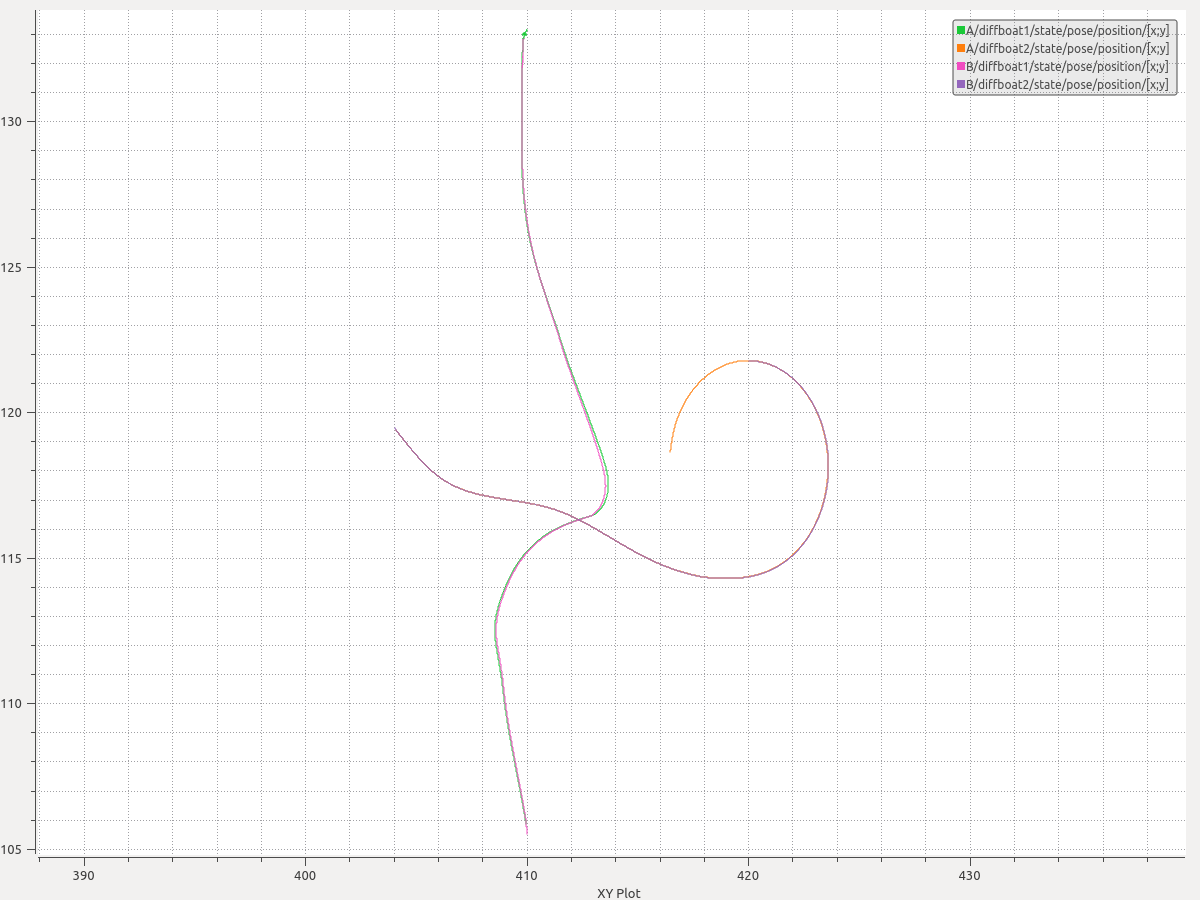
\includegraphics[width=\textwidth]{figs/Chap5/plot_cl_w_vs_wo.png}
                \caption{Trajectory}
                \label{fig:plot_cl_w_vs_wo}
            \end{subfigure}
            \begin{subfigure}[b]{0.49\textwidth}
                \centering
                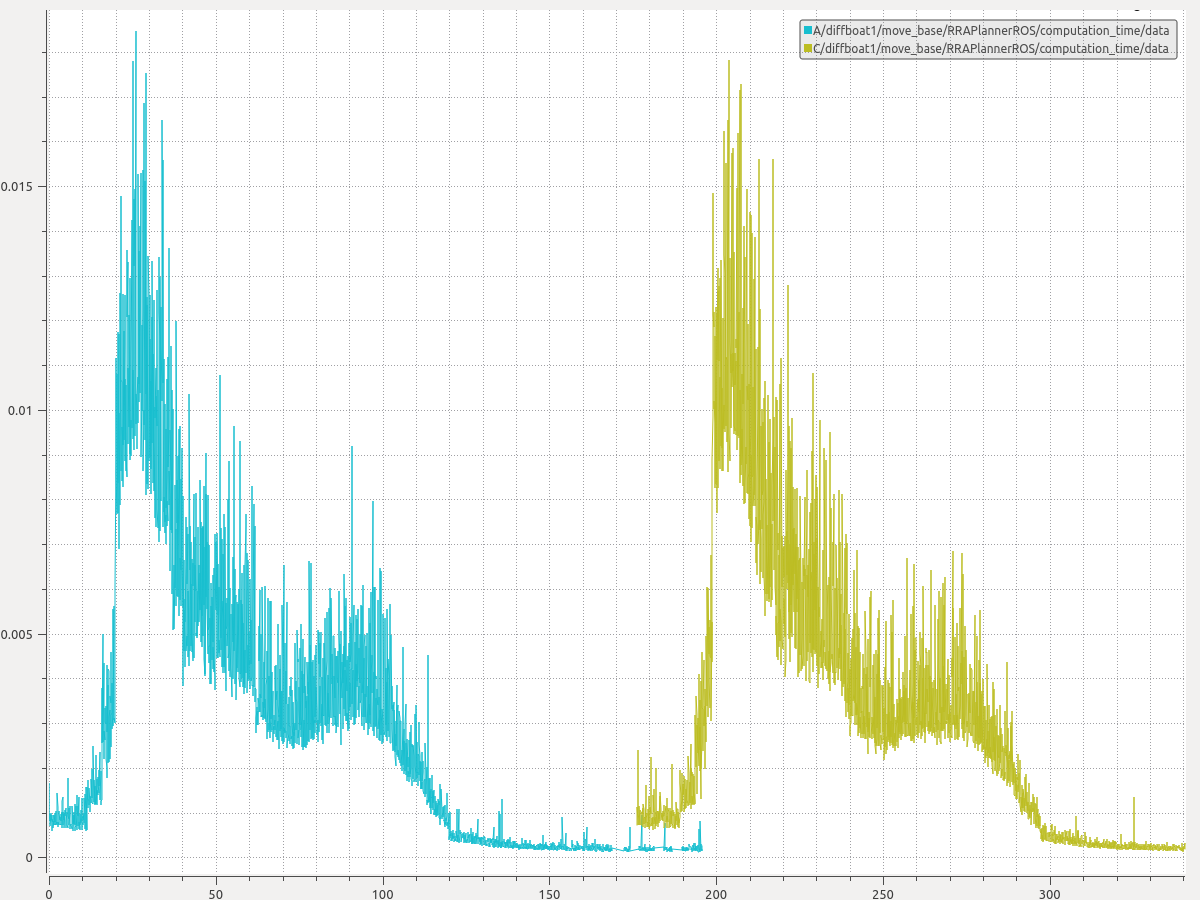
\includegraphics[width=\textwidth]{figs/Chap5/plot_cl_w_vs_wo_CT.png}
                \caption{Computation Time}
                \label{fig:plot_cl_w_vs_wo_CT}
            \end{subfigure}
            
            \begin{subfigure}[b]{0.49\textwidth}
                \centering
                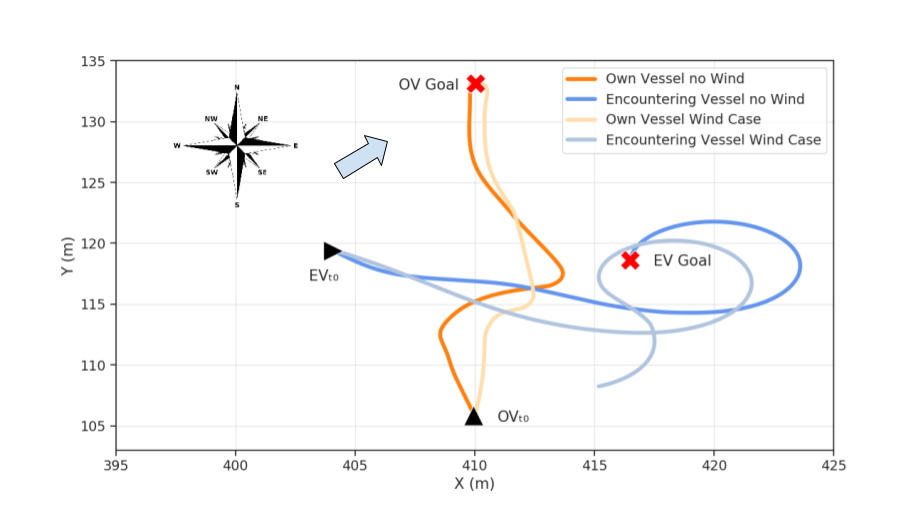
\includegraphics[width=\textwidth]{figs/Chap5/plot_cl_w_vs_wind.png}
                \caption{Trajectory}
                \label{fig:plot_cl_w_vs_wind}
            \end{subfigure}
            \begin{subfigure}[b]{0.49\textwidth}
                \centering
                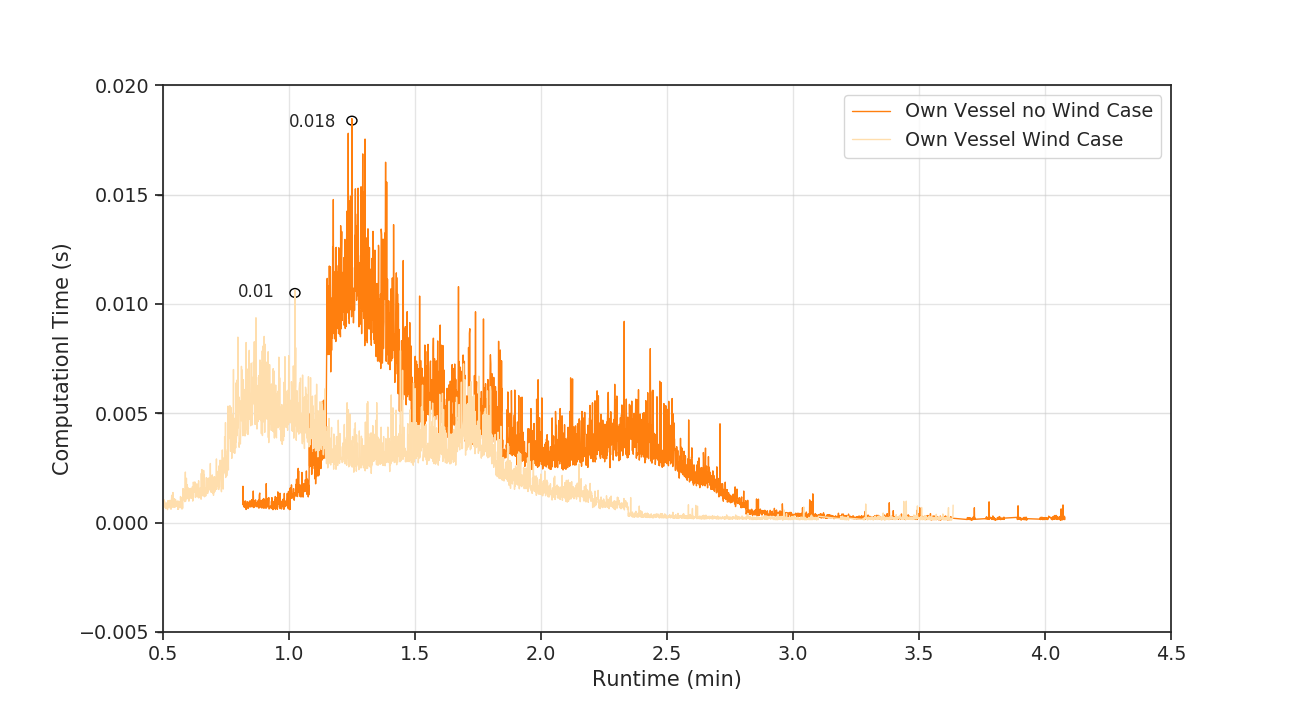
\includegraphics[width=\textwidth]{figs/Chap5/plot_cl_w_vs_wind_CT.png}
                \caption{Computation Time}
                \label{fig:plot_cl_w_vs_wind_CT}
            \end{subfigure}
        
        \caption{Crossing Right Encounter Scenario. Comparing \ac{ATC} versus no \ac{ATC} cases and, with and Wind vs no Wind cases.}
        \label{fig:plots_cl}
        \end{figure}
        
        %%%%%%%%%%%%%%%%%%%%%%%%%%%%%%%%%%%%%%
        %% Overtaking w vs wo \ac{ATC}. w vs wo Wind
        %
        %% Grammarlly: 100/100
        %%%%%%%%%%%%%%%%%%%%%%%%%%%%%%%%%%%%%%
        In Figure \ref{fig:plots_ov}, we present the behavior of our system when \ac{OV} encounters another vessel coming from the right. In Figure \ref{fig:plot_ov_w_vs_wo} we show the comparison between trajectories with and without ATC and in Figure \ref{fig:plot_ov_w_vs_wo} we can see computational time for each case. As we can see, once again, our method implies COLREGS compliance when avoiding a collision. In Figure \ref{fig:plot_ov_w_vs_wind} we show the comparison between trajectories with and without wind influence and in Figure \ref{fig:plot_ov_w_vs_wind_CT} we can see computational time for each case. 
        \begin{figure}[H]
        \centering
        
            \begin{subfigure}[b]{0.49\textwidth}
                \centering
                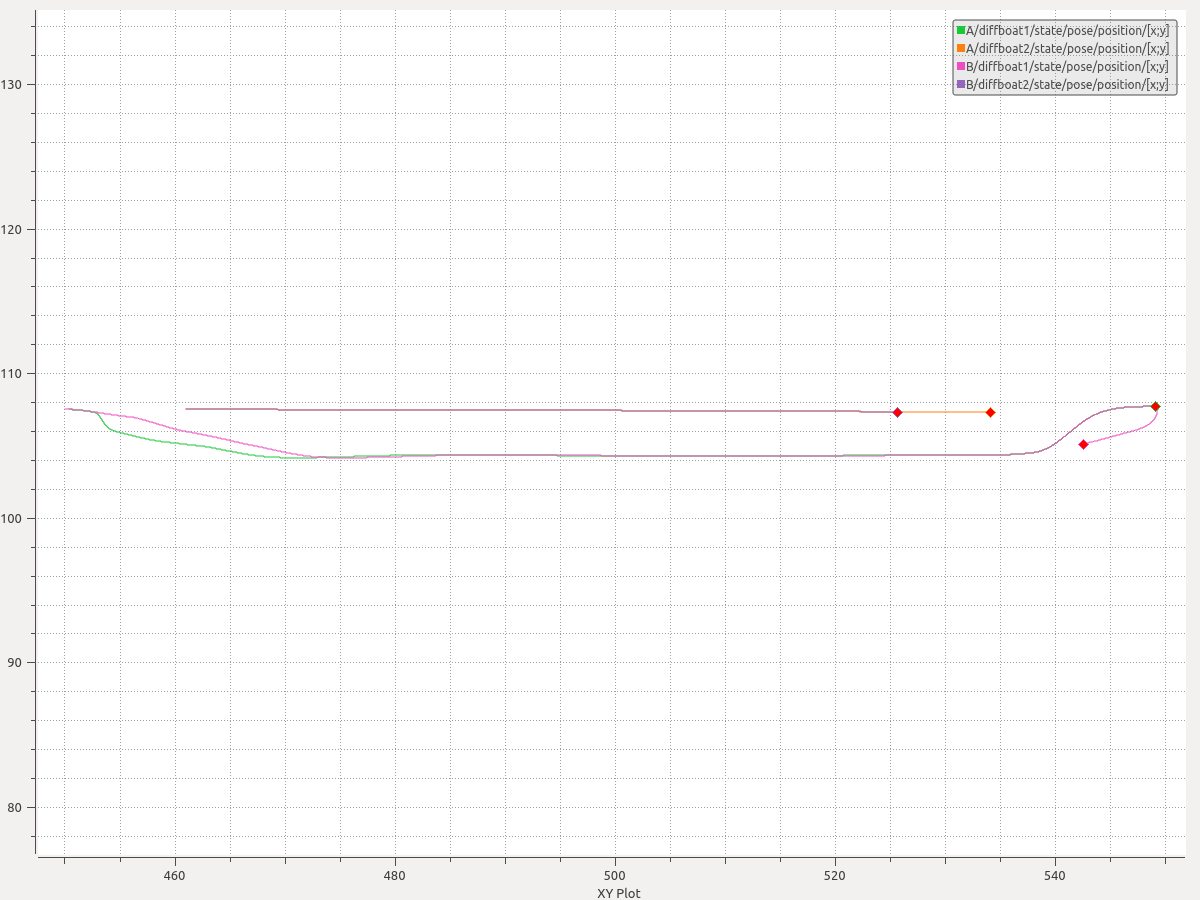
\includegraphics[width=\textwidth]{figs/Chap5/plot_ov_w_vs_wo.png}
                \caption{Trajectory}
                \label{fig:plot_ov_w_vs_wo}
            \end{subfigure}
            \begin{subfigure}[b]{0.49\textwidth}
                \centering
                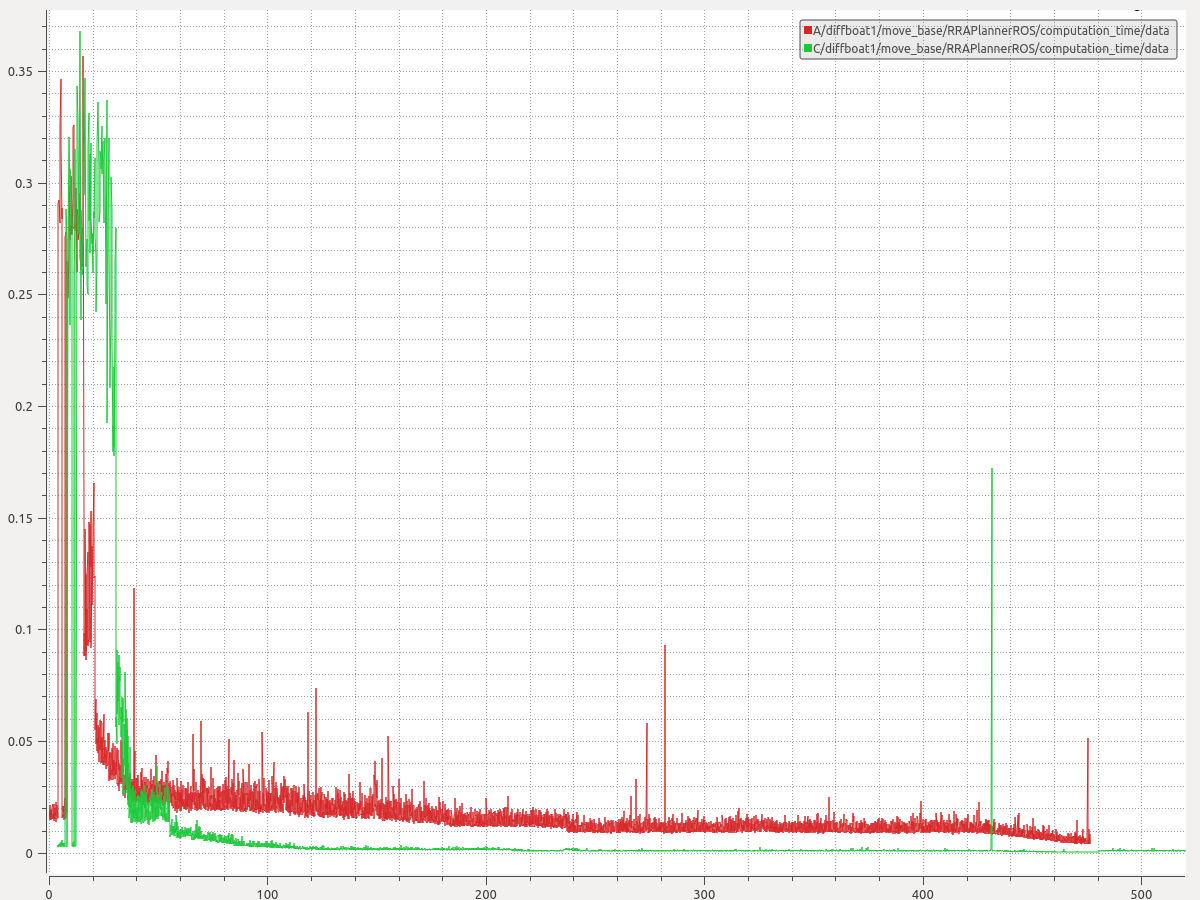
\includegraphics[width=\textwidth]{figs/Chap5/plot_ov_w_vs_wo_CT.png}
                \caption{Computation Time}
                \label{fig:plot_ov_w_vs_wo_CT}
            \end{subfigure}
            
            \begin{subfigure}[b]{0.49\textwidth}
                \centering
                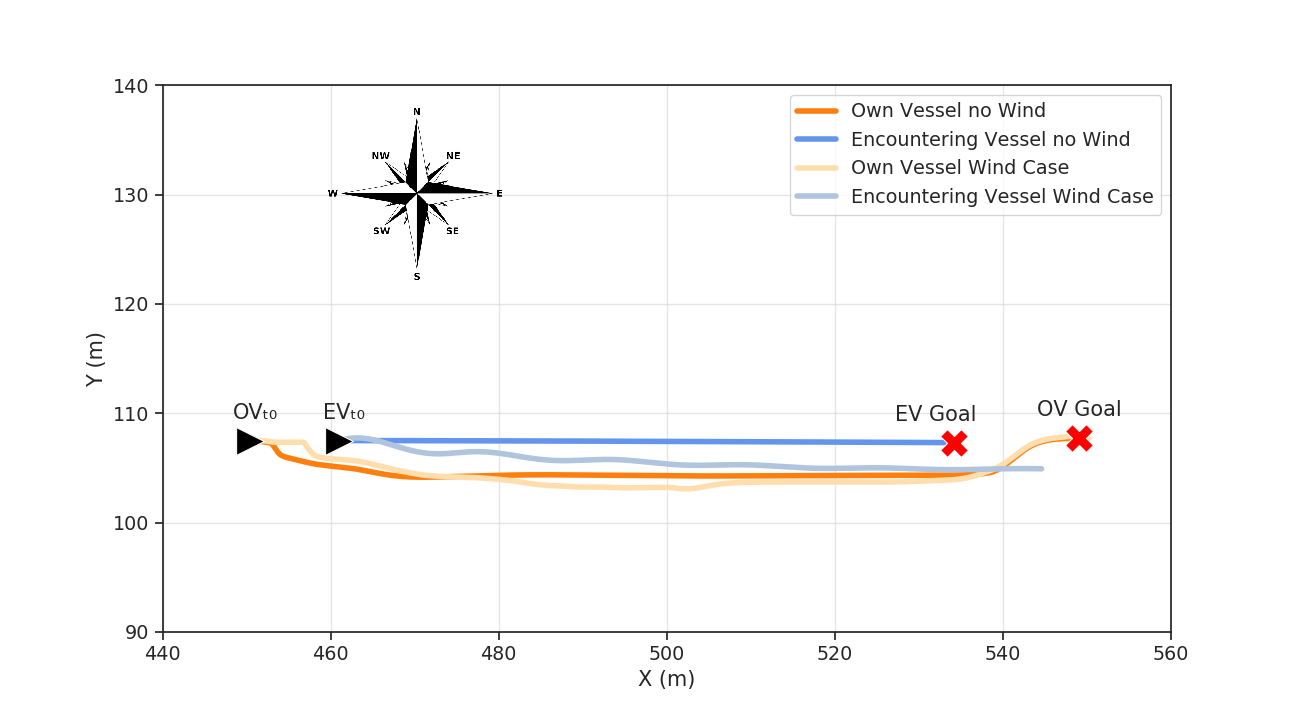
\includegraphics[width=\textwidth]{figs/Chap5/plot_ov_w_vs_wind.png}
                \caption{Trajectory}
                \label{fig:plot_ov_w_vs_wind}
            \end{subfigure}
            \begin{subfigure}[b]{0.49\textwidth}
                \centering
                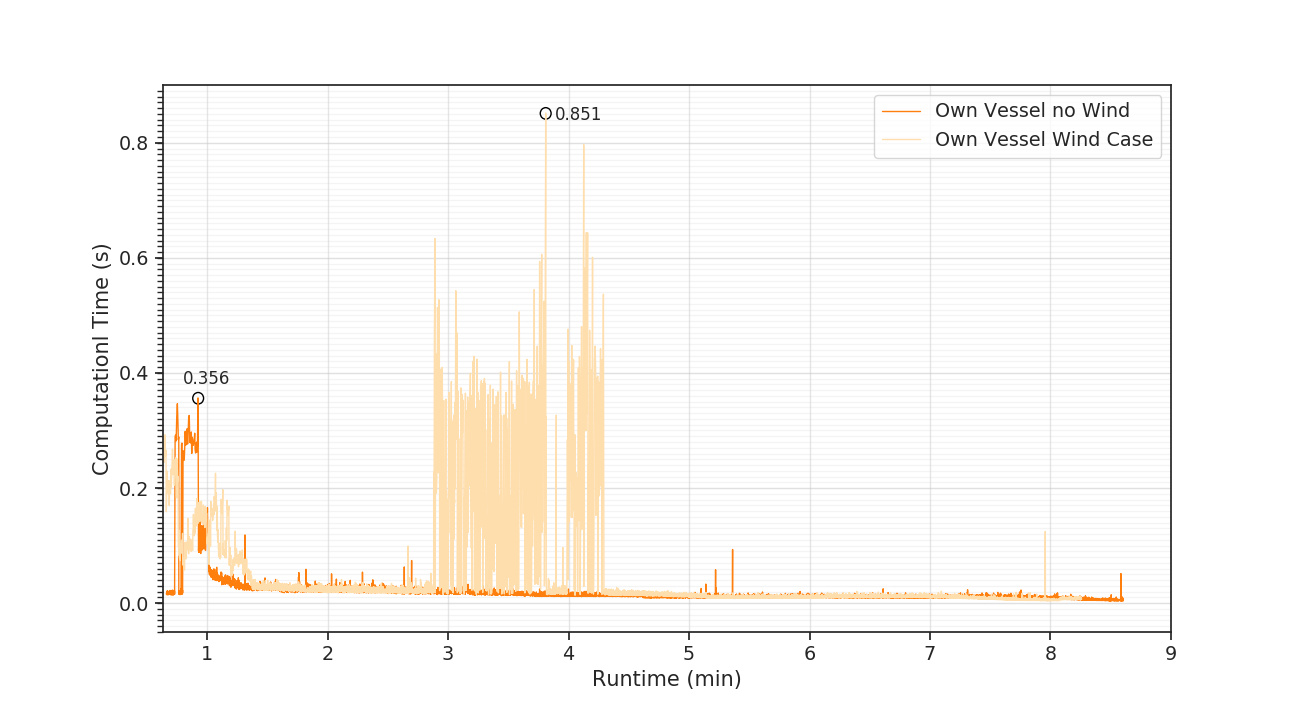
\includegraphics[width=\textwidth]{figs/Chap5/plot_ov_w_vs_wind_CT.png}
                \caption{Computation Time}
                \label{fig:plot_ov_w_vs_wind_CT}
            \end{subfigure}
        
        %% Grammarlly: 98/100
        \caption{Overtaking Encounter Scenario with \ac{ATC}, with and without wind. In \ref{fig:plot_ov_w_vs_wind_CT} we can see a considerable increase in computation time from around 3 minutes until aorund 4min and 25 second. This happened due to the second limitation discovered in our method. With \ac{ATC} the creation of virtual obstacles can be conflicting with the A* goal location and its neighbors, in this situation the planner is not able to decide the route to be followed and decided to use the last generated speed command until the position of the A* goal location is free. Due to the conflicting position of the created virtual obstacle and local A* goal, the computational time cost achieves great value, since it explored the whole search space and found no solution.}
        \label{fig:plots_ov}
        \end{figure}
        
        %% Grammarlly: 100/100
        In Table \ref{tab:results}, we summarize the results for the different simulations we have done. In simulation scenarios, we can see that the computational time peak keeps in a range from 0.355 to 0.390 for no \ac{ATC} configuration, from 0.357 to 0.395 for \ac{ATC} configuration and from 0.355 to 0.8852 for Wind configuration. Computation time for no \ac{ATC} and \ac{ATC} are similar since our \ac{ATC} method has a low impact on the A* implementation. With the influence of wind, we see an increase in the computational time peak. For the Overtaking scenario, the influence of wind caused our system to an exhaustive scenario search in the whole search space.
        
        %% Grammarlly: 100/100
        The average time keeps similar for each scenario encounter, not depending on the configuration (no \ac{ATC}, \ac{ATC}, and Wind) and consumed at least 4.6 times less time. Regarding minimum distance, in our simulations, our system kept at least a safe distance of 1.505 meters from \ac{EV}. \ac{COLREGS} do not specify a specific value for safe distance or a proportion related to \ac{OV}'s size, but for some authors \cite{} \acp{USV} should at least keep a safe distance as the size of the vessel.
    
%AMA a diferenca entre avg e max eh enorme. explique bem o motivo disso. p um problema de tempo real, essa variacao nao eh muito interessante. 
%: 

\begin{table}
\caption{Based on \cite{Lazarowska2017New, Singh2018Constrained, Agrawal2015COLREGS, Candeloro2017Voronoi, Svec2013Dynamics} we made a quantitative evaluation of our planning system measuring computational cost and the minimum distance kept between the vessels during simulations.}
\label{tab:results}
\centering
\begin{tabular}{ccccccc} 
\toprule
\multirow{2}{*}{\begin{tabular}[c]{@{}c@{}}\textbf{Encounter}\\\textbf{Type} \end{tabular}}     & \multirow{2}{*}{\textbf{Case} } & \multicolumn{3}{c}{\textbf{Computational Time (s)} }          & \multirow{2}{*}{\begin{tabular}[c]{@{}c@{}}\textbf{Successful }\\\textbf{Avoidance }\end{tabular}} & \multirow{2}{*}{\begin{tabular}[c]{@{}c@{}}\textbf{Minimum }\\\textbf{Distance (m) }\end{tabular}}  \\ 
\cmidrule[\heavyrulewidth]{3-5}
                                                                                                &                                 & \textbf{Maximum} & \textbf{Average} & \textbf{Std. Variation} &                                                                                                    &                                                                                                     \\ 
\toprule
\multirow{3}{*}{\textbf{Head-On}}                                                               & \textbf{No ATC}                 & 0.369            & 0.074            & 0.081                   & Yes                                                                                                & 4.431                                                                                               \\
                                                                                                & \textbf{ATC}                    & 0.364            & 0.076            & 0.076                   & Yes                                                                                                & 1.599                                                                                               \\
                                                                                                & \textbf{Wind}                   & 0.355            & 0.077            & 0.079                   & Yes                                                                                                & 1.505                                                                                               \\ 
\cline{2-7}
\multirow{3}{*}{\begin{tabular}[c]{@{}c@{}}\textbf{Crossing}\\\textbf{from Right}\end{tabular}} & \textbf{No ATC}                 & 0.390            & 0.050            & 0.098                   & Yes                                                                                                & 5.414                                                                                               \\
                                                                                                & \textbf{ATC}                    & 0.390             & 0.052            & 0.104                   & Yes                                                                                                & 3.264                                                                                               \\
                                                                                                & \textbf{Wind}                   & 0.403            & 0.085            & 0.124                   & Yes                                                                                                & 3.739                                                                                               \\ 
\cline{2-7}
\multirow{3}{*}{\begin{tabular}[c]{@{}c@{}}\textbf{Crossing}\\\textbf{from Left}\end{tabular}}  & \textbf{No ATC}                 & 0.018                 & 0.003                 & 0.003                        &  Yes                                                                                                  & 1.345                                                                                                    \\
                                                                                                & \textbf{ATC}                    & 0.018                 & 0.003                 & 0.003                        & Yes                                                                                                   & 1.364                                                                                                    \\
                                                                                                & \textbf{Wind}                   & 0.011                 & 0.002                 & 0.002                        & Yes                                                                                                   & 0.790                                                                                                    \\ 
\cline{2-7}
\multirow{3}{*}{\textbf{Overtaking}}                                                            & \textbf{No ATC}                 & 0.368            & 0.006            & 0.030                   & Yes                                                                                                & 3.325                                                                                               \\
                                                                                                & \textbf{ATC}                    & 0.357            & 0.018            & 0.022                   & Yes                                                                                                & 3.101                                                                                               \\
                                                                                                & \textbf{Wind}                   & 0.852            & 0.039            & 0.073                   & Yes                                                                                                & 1.787                                                                                               \\
\bottomrule
\end{tabular}
\end{table}